\chapter{Biblioteka EPUBKit}

Tworzenie biblioteki, którą zamierzamy następnie wykorzystać we własnej aplikacji lub udostępnić publiczne, jest stosunkowo prostym rozwiązaniem. Wszystko sprowadza się do stworzenia nowego projektu w Xcode, a następnie dołączenie go do przestrzeni roboczej (Xcode Workspace) w której znajdzie się projekt aplikacji nad którą pracujemy oraz projekt biblioteki. Aby stworzyć projekt biblioteki należy uruchomić Xcode IDE i na powitalnym ekranie wybrać opcję \textit{Create a new Xcode project}, która przeniesie nas do kolejnego ekranu z możliwością wybrania konkretnego szablonu projektu nad jakim chcemy pracować, tak jak jest to zaprezentowane na ilustracji \ref{chapter-4-image-1-new-project}.

\begin{figure}[ht!]
  \centering
  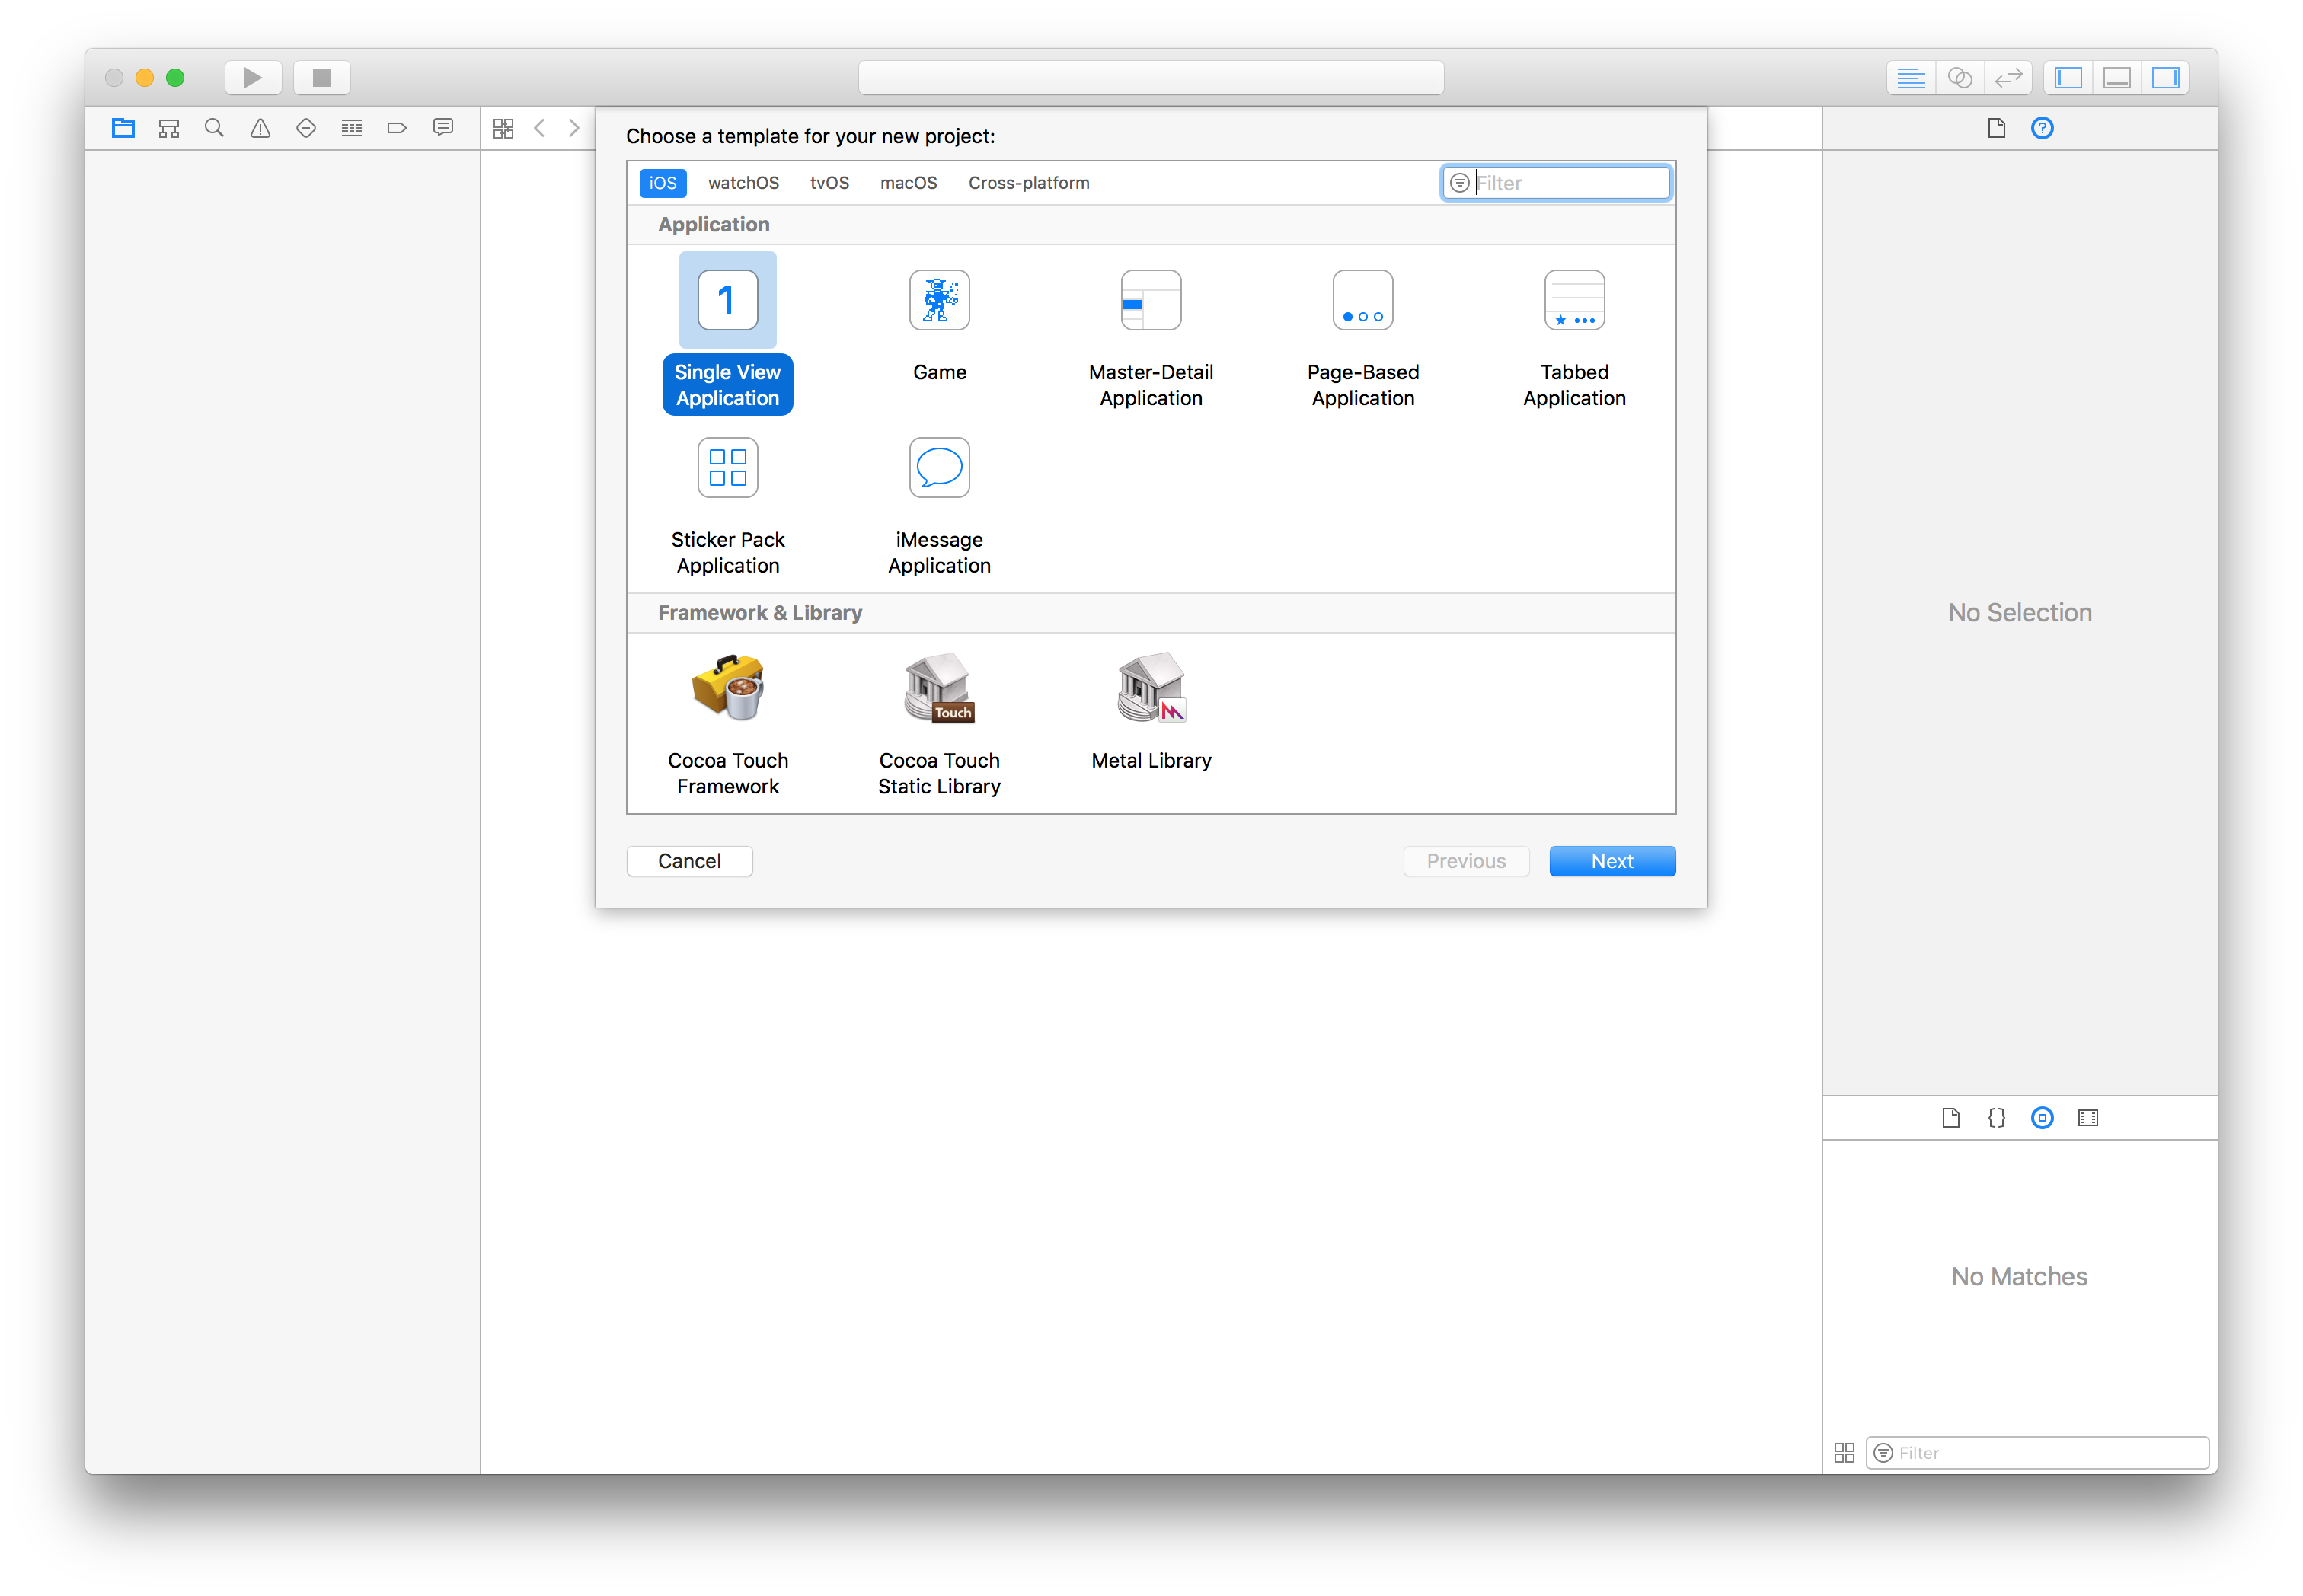
\includegraphics[width=120mm]{images/chapter-4-image-1-new-project.png}
  \caption{Szablny projektów które znajdują się w Xcode}
  \label{chapter-4-image-1-new-project}
\end{figure}

W naszym przypadku interesuje nas szablon \textit{Cocoa Touch Framework}, a po jego wybraniu jesteśmy proszeni o uzupełnienie formularza ze szczegółowymi informacjami na temat projektu, który zamierzamy stworzyć, poczynając od nazwy, po język w którym będzie napisany, tj. Swift lub Objective-C. Następnie Xcode poprosi o wskazanie lokalizacji na dysku, w której chcemy zapisać projekt, oraz zapyta nas czy chcemy stworzy repozytorium systemu kontroli wersji git. W tym momencie mamy projekt, który można już w prosty sposób dołączyć do aplikacji. Zostanie to dokładnie opisane w kolejnym rozdziale przy okazji omawianie wykorzystania biblioteki EPUBKit w demonstracyjnej aplikacji. Teraz już możemy tworzyć klasy, które mają składać się na funkcjonalność biblioteki.

\begin{figure}[ht!]
  \centering
  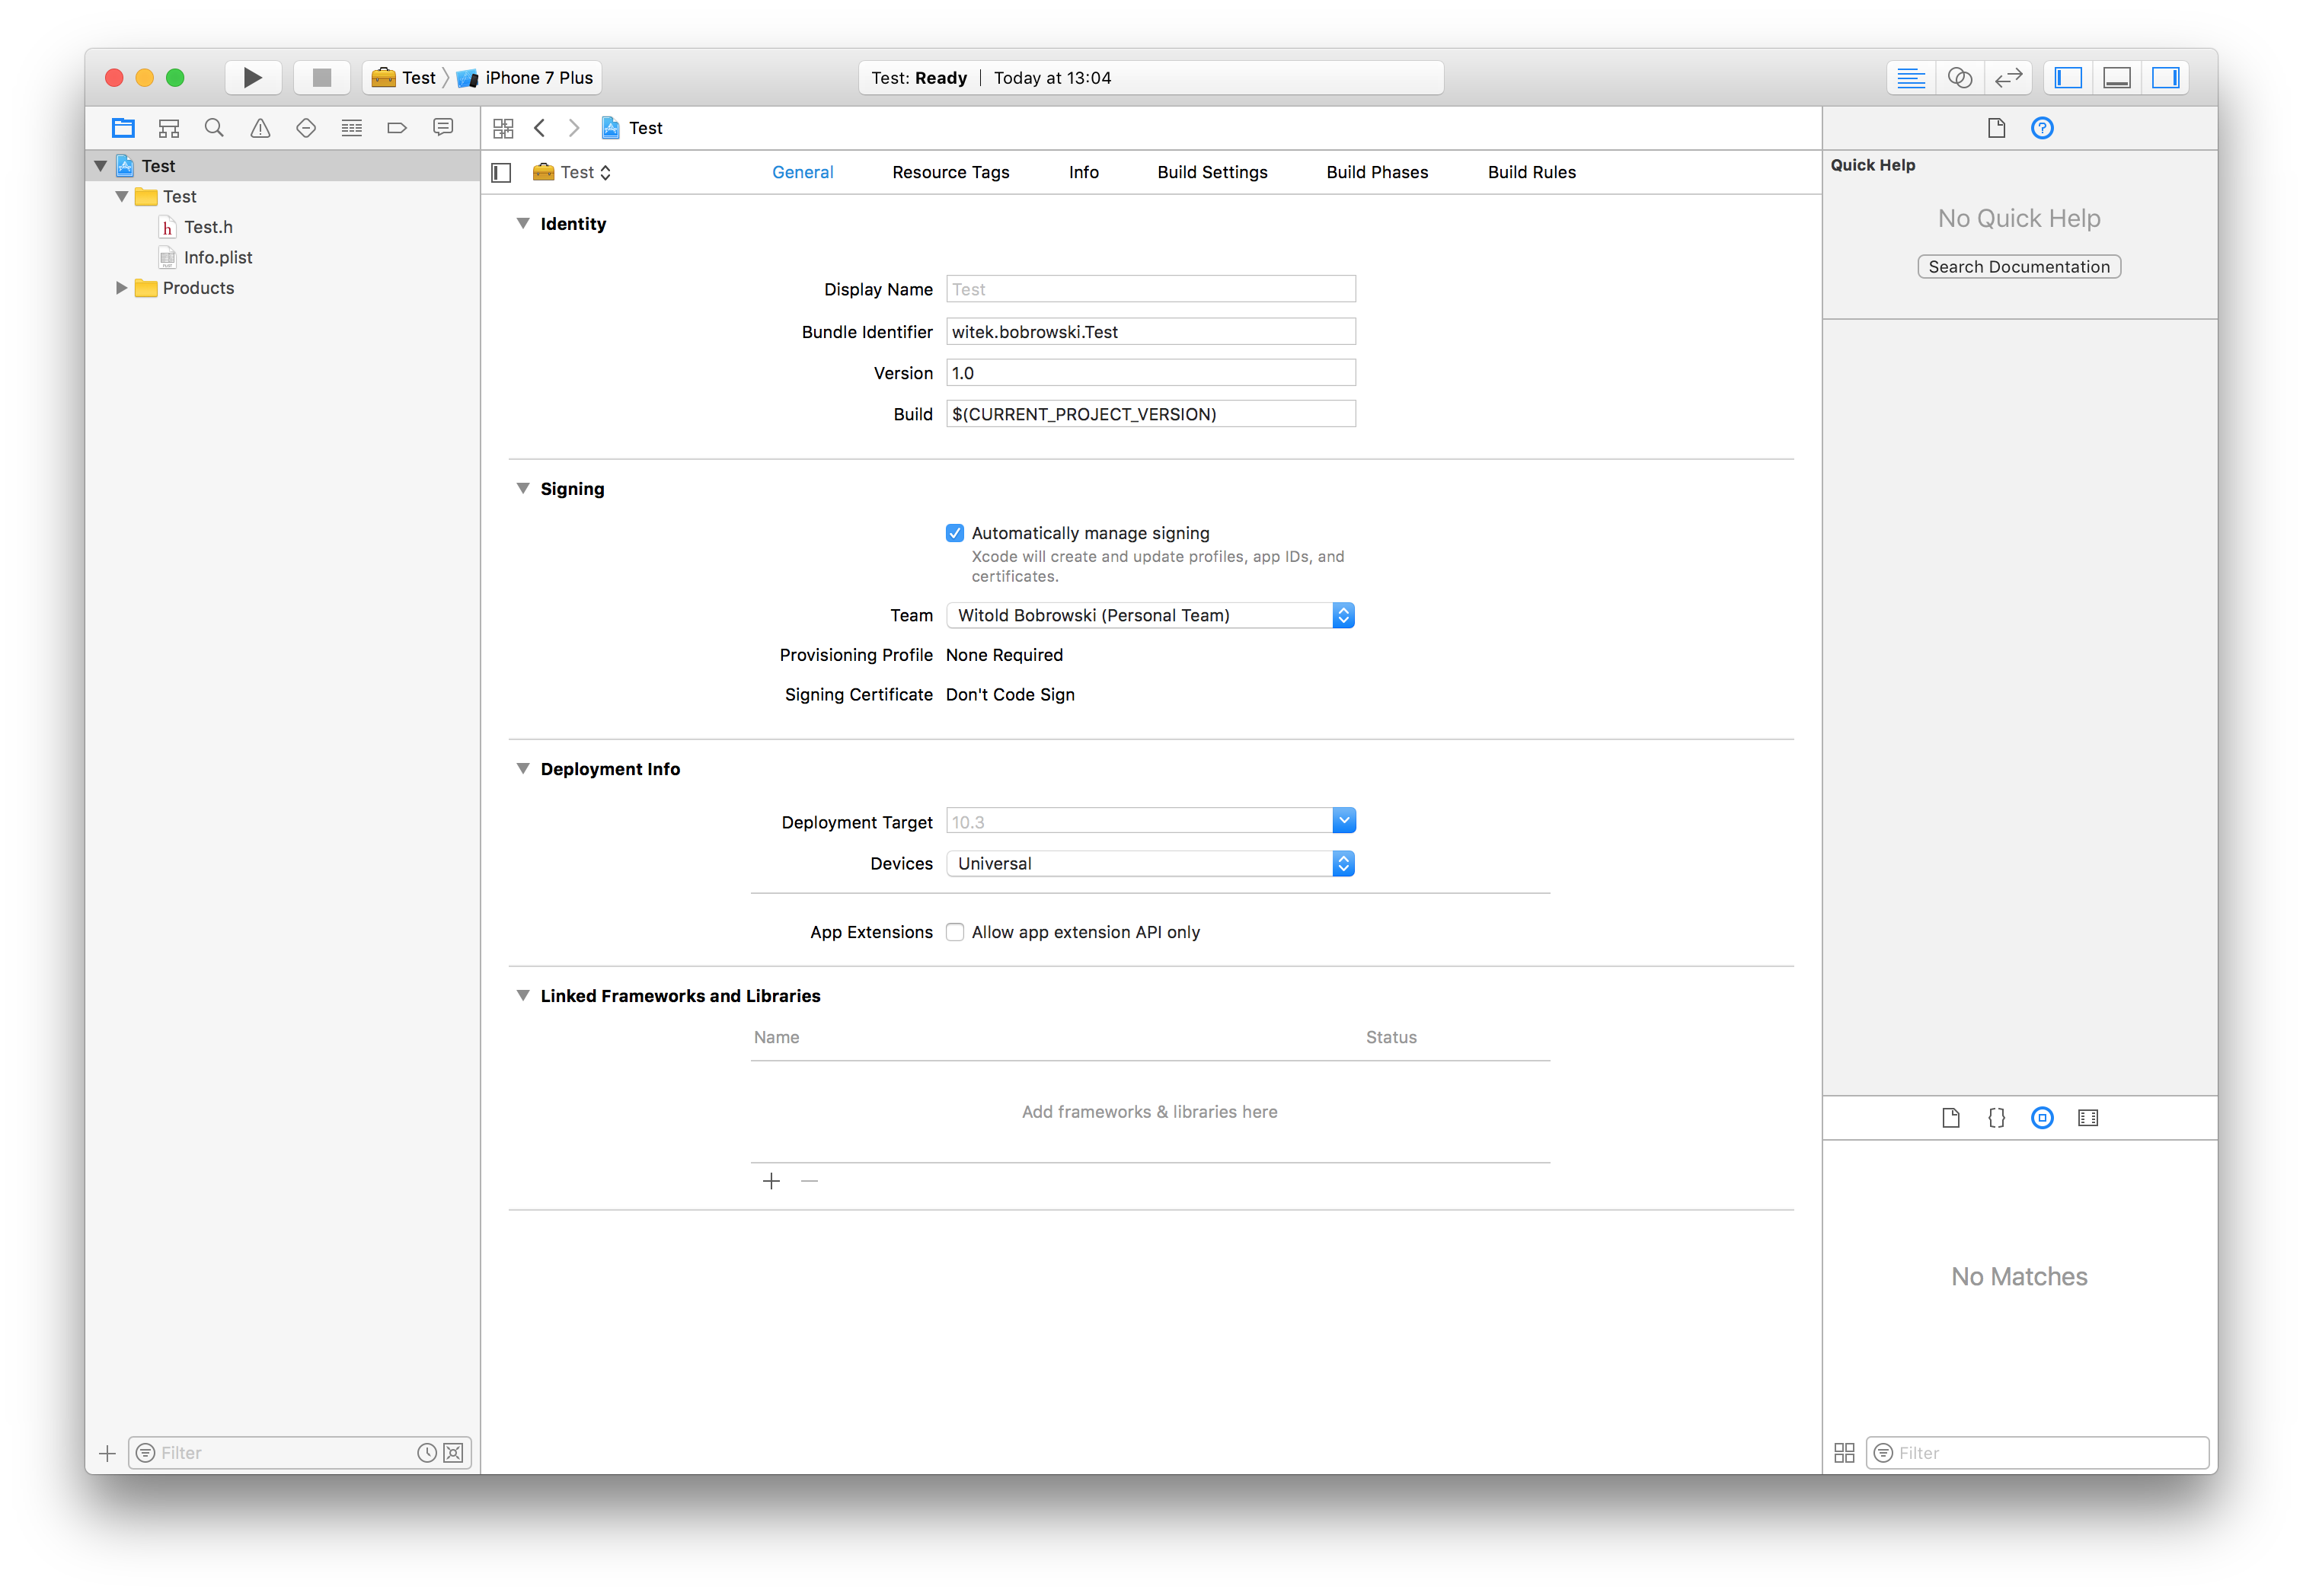
\includegraphics[width=120mm]{images/chapter-4-image-2-empty-project.png}
  \caption{Widok nowego, pustego projektu}
  \label{chapter-4-image-2-empty-project}
\end{figure}

Plik projektu, którego widok jest widoczny na ilustracji \ref{chapter-4-image-2-empty-project} pozwala nam na szczegółowy wgląd w preferencje oraz informacje jego dotyczące, które można zmienić w dowolnej chwili. Jest możliwość zmiany wersji biblioteki, docelowego urządzenia, preferowanej wersji systemu który ma wspierać biblioteka, oraz co bardzo istotne, mamy możliwość użycia innych niezależnych bibliotek w naszym projekcie. Wystarczy wyeksportować plik projektu jako plik przestrzeni roboczej do której można dodać inne projekty, a następnie połączyć je z naszym w menu \textit{General} w polu \textit{Linked Frameworks and Libraries} w pliku projektu. Dzięki tak funkcjonalnym i prostym w obsłudze narzędziom jak Xcode, po szybkiej konfiguracji swoją uwagę można skupić na samej logice którą chcemy zaimplementować.

W tym rozdziale zostanie opisana stworzona przez mnie biblioteka EPUBKit. Biblioteka ta jest oparta na architekturze MVC (Model View Controller), dlatego omówienie zaczyna się od opisania jej modelu oraz parsera, a następnie przejdę do zawartych w niej widokach, które pozwalają na wyświetlenie danych zawartych w modelu. Zakończę rozdział przedstawiając możliwości dystrybuowania takiej biblioteki, przy pomocy szeroko stosowanych i popularnych narzędzi, które są podstawą programowania na platformę iOS.

\section{Model}

Struktura klas modelu zaprezentowana na wykazie \ref{model-organization}, została zaprojektowana w ten sposób, aby z jednej strony odzwierciedlała strukturę dokumentu EPUB oraz format OPF który EPUB wykorzystuje, a z drugiej by trzymała się konwencji ,,swiftowych'' i intuicyjnie reprezentowała instancję, która następnie będzie wykorzystana w kolejnych klasach biblioteki.

\begin{lstlisting}[caption={Struktura modelu EPUBKit}, language=bash,label=model-organization]
Model
|-- EPUBDocument.swift
|-- EPUBManifest.swift
|-- EPUBMetadata.swift
|-- EPUBSpine.swift
`-- EPUBTableOfContents.swift
\end{lstlisting}

\subsection{EPUBDocument}
\label{EPUBDocument}

EPUBDocument jest klasą publiczną reprezentującą całą publikację EPUB i agregującą pozostałe struktury modelu biblioteki jako jej stałe własności. Ze względu na nomenklaturę stosowaną w języku Swift, \textit{properties} będą nazywane własnościami). Tak jak przedstawiono na wykazie \ref{propety-declaration}, w języku Swift odróżniamy dwa rodzaje własności, są to stałe \texttt{let} do których wartość może zostać przypisana wyłącznie jednokrotnie oraz zmienne \texttt{var} których wartość może być modyfikowana w dowolnym momencie.

\begin{lstlisting}[caption={Deklaracje własności w Swifcie.\cite{theSwiftProgrammingLanguageDeclarations}}, language=swift-reference,label=propety-declaration]
 let (constant name): (type) = (expression)
 var (variable name): (type) = (expression)
\end{lstlisting}

Własności zostały oznaczone jako stałe ze względu na statyczną naturę struktury publikacji EPUB. Ciężko sobie wyobrazić powód dla którego któreś z metadanych publikacji miały by zostać zmienione albo któreś z dokumentów XML usunięte z manifestu publikacji. Dlatego biorąc pod uwagę kontekst, w którym klasa się znajduje, zdecydowałem się oznaczenie jej własności jako stałe, co jest widoczne na wykazie \ref{EPUBDocument-declaration}, aby zapewnić klasie niemodalność oraz zgodność z wytycznymi odnośnie projektowania klas i struktur w języku Swift, według których powinno oznaczać się własności jako stałe w każdej sytuacji, która nie wymaga od nas ich mutowania. Słowa ,,mutowania'' użyłem tutaj nie bez powodu, co stanie się jasne w kolejnym akapicie.

\begin{lstlisting}[caption={Klasa EPUBDocument i jej stałe publiczne}, language=swift,label=EPUBDocument-declaration]
public class EPUBDocument {
    public let directory: URL
    public let contentDirectory: URL
    public let metadata: EPUBMetadata
    public let manifest: EPUBManifest
    public let spine: EPUBSpine
    public let tableOfContents: EPUBTableOfContents
}
\end{lstlisting}

W przeciwieństwie do C, struktury w Swiftcie mogą posiadać metody. W przypadku, gdy metoda w jakiś sposób zmienia własności, musi ona zostać oznaczona słowem kluczowym \texttt{mutating} co tyczy się również metod enumeracji. Wspominam o tym, ponieważ chciałbym wytłumaczyć dlaczego typy własności klasy \texttt{EPUBDocument} są strukturami, a nie klasami. Ze względu na to, że instancje klasy są przekazywane przez referencję, a instancje struktur są przekazywane przez kopiowanie wartości, oznacza to że są one przeznaczone do innych zadań. Zgodnie z wytycznymi Apple, strukturami powinno oznaczać się typy, których zadaniem jest enkapsulacja relatywnie prostych wartości \cite{theSwiftProgrammingLanguageStructsPurpose}, co jest prawdą w przypadku wcześniej wspomnianych typów, a które zostaną one opisane w kolejnych paragrafach.

Klasa \texttt{EPUBDocument} posiada dwa inicjalizatory widoczne na wykazie \ref{EPUBDocument-initializers}, które pozwalają tworzyć instancje tej klasy. Pierwszym z nich jest inicjalizator prywatny w nomenklaturze swiftowej \textit{memberwise initializer} ze względu na kolejność argumentów które przyjmuje. Jest ona zgodna  z kolejnością deklaracji własności. Inicjalizator ten został oznaczony jako prywatny, ponieważ jego przeznaczeniem jest inicjalizować instancję jedynie przy pomocy drugiego inicjalizatora. Drugi z inicjalizatorów jest dostępny publicznie i jest jedynym publicznym inicjalizatorem dla tej klasy.

\begin{lstlisting}[caption={Inicjalizatory klasy EPUBDocument}, language=swift,label=EPUBDocument-initializers]
private init (directory: URL, contentDirectory: URL, metadata: EPUBMetadata, manifest: EPUBManifest, spine: EPUBSpine, toc: EPUBTableOfContents) {
    self.directory = directory
    self.contentDirectory = contentDirectory
    self.metadata = metadata
    self.manifest = manifest
    self.spine = spine
    self.tableOfContents = toc
}

public convenience init?(named: String) {
    let parser = try? EPUBParser(named: named)
    guard let directory = parser?.directory,
        let contentDirectory = parser?.contentDirectory,
        let metadata = parser?.metadata,
        let manifest = parser?.manifest,
        let spine = parser?.spine,
        let tableOfContents = parser?.tableOfContents else { return nil }
    self.init(directory: directory, contentDirectory: contentDirectory, metadata: metadata, manifest: manifest, spine: spine, toc: tableOfContents)
}
\end{lstlisting}

Zważając na naturę publikacji EPUB jako spójnej całości, zdecydowałem ograniczyć się inicjalizowanie klasy \texttt{EPUBDocument} do inicjalizatora pomocniczego, który wykorzystuje do tego parser. Ten inicjalizator wykorzystuje w pełni możliwości Swifta. Oznaczając go słowem kluczowym \textit{convenience}, zmuszam go do wykorzystania wyznaczonego (ang. designated) inicjalizatora, ponieważ pomocniczy inicjalizator nie może samemu tworzyć instancji, musi do tego wykorzystać wyznaczony inicjalizator. W tym przypadku jest to pierwszy inicjalizator, który jest prywatny. Dodatkowo pomocniczy inicjalizator, jest oznaczony znakiem zapytania \texttt{init?} co oznacza, że inicjalizacje może się nie powieść, a w takiej sytuacji inicjalizator zwróci\ldots nic, czyli \texttt{nil} w Swifcie. Konsekwencją tego jest to, że typ który zwraca ten inicjalizator to \texttt{EPUBDocument?}, a nie \texttt{EPUBDocument}, co oznacza że może on nie mieć żadnej wartości, co trzeba w odpowiedni sposób obsłużyć. Przeanalizujmy więc krok po kroku operacje, które wykonuje inicjalizator pomocniczy.

\begin{lstlisting}[language=swift-reference,caption={Inizjalizacja EPUBParser},label={epub-init-1}]
let parser = try? EPUBParser(named: named)
\end{lstlisting}

Inicjalizator zaczynając od instrukcji widocznej na wykazie \ref{epub-init-1}, tworzy instancję parsera, i jako argument inicjalizatora podaje własny parametr który wskazuje na nazwę publikacji EPUB. Słowo kluczowe \texttt{try} oznacza, że inicjalizator może zwrócić błąd, a dzięki znakowi zapytania błąd ten gdy zostanie rzucony, będzie interpretowany jako zwrócenie wartości \texttt{nil} przez inicjalizator. W ten sposób unikamy umieszczenia bloku \texttt{do-catch}, co znacznie upraszcza kod. Na końcu znajdujemy się w posiadaniu stałej \texttt{parser}, która jest typu \texttt{EPUBParser?} czyli opcjonalny \texttt{EPUBParser}.

\begin{lstlisting}[language=swift-reference,caption={Wyrażenie \texttt{guard let}},label={epub-init-2}]
guard let directory = ... else { return nil }
\end{lstlisting}

Wyrażenie \texttt{guard let} przedstawione na wykazie \ref{epub-init-2} jest jednym ze sposobów obsłużenia typu opcjonalnego. Jest to odmiana wyrażenia \texttt{if let}, które pozwala nam na przypisanie wartości zmiennej \texttt{a}, do nowej stałej \texttt{b}, jeżeli zmienna \texttt{a} takową posiada. Wadą takiego rozwiązania jest to, że nowo powstała zmienna \texttt{b}, znajduje się jedynie w zasięgu bloku \texttt{if}, co w pewien sposób ogranicza dostęp do niej. Z pomocą przychodzą wyrażenia \texttt{guard}, dzięki którym zadeklarujemy nową stałą, która będzie przyjmowała wartość zmiennej, którą chcemy \textit{rozpakować} (ang. unwrap -- co odnosi się do czynności wywłaszczania wartości z typu opcjonalnego) i będzie ona dostępna w obrębie tego samego bloku co wyrażenie \texttt{guard}. Dodatkowo mamy możliwość wykonania jakiejś czynności w sytuacji gdy zmienna, którą rozpakowujemy nie ma wartości, co w tym konkretnym przypadku będzie oznaczało niepowodzenie wywłaszczenia którejś z wartości parsera, a więc inicjalizator \texttt{EPUBDocument} zwróci \texttt{nil}. Wyrażenie \texttt{guard} działa w podobny sposób co \texttt{if}, dlatego otrzymuje on również te same funkcjonalności co \texttt{if} w Swifcie, czyli możliwość kolejkowania wyrażeń zwracających wartość boolowską, tj. wypisujemy je kolejno po przecinku. W przypadku zwrócenia fałszu przez jedno z nich, instrukcja natychmiast zostaje przerwana, a pozostałe wyrażenia nie zostają ewaluowane. W tym przypadku program przechodzi do bloku \texttt{else}.

\begin{lstlisting}[language=swift-reference,caption={Inicjalizaca danymi z parsera},label={epub-init-3}]
self.init(...)
\end{lstlisting}

Jeżeli udało się wywłaszczyć wszystkie potrzebne wartości z parsera, to można przejść do tworzenia instancji \texttt{EPUBDocument}. Inicjalizator pomocniczy wywołuje inicjalizator wyznaczony(wykaz \ref{epub-init-3}), i dokument zostaje pomyślnie stworzony, a wszystkie informacje otrzymane dzięki parserowi zostają przypisane na stałe do jednej instancji \texttt{EPUBDocument}. W ten sposób zostaje zachowana niemutowalność instancji oraz gwarancja, że wszystkie wartości w których posiadaniu znajduje się instancja, pochodzą z jednego źródła, z którego czerpie parser. Omówienie działanie samego parsera zostawiam na kolejny podrozdział.

\subsection{EPUBManifest}

Jak już wspomniano w rozdziale opisującym format EPUB, jego struktura jest oparta o standard OPF a to oznacza, że znajduje się w nim wykaz (manifest) wszystkich dokumentów oraz zasobów na które składa się dokument. Każdy element wymieniony w manifeście posiada swoje ID, wskazaną ścieżkę w strukturze dokumentu oraz typ. Parser starannie analizuje manifest i tworzy strukturę w której posiadaniu następnie znajduje się instancja \texttt{EPUBDocument}, o czym więcej przy okazji omawiania parsera.

\begin{lstlisting}[caption={Struktura EPUBManifest}, language=swift,label=EPUBManifest-declaration]
public struct EPUBManifest {
    public struct Item {
        public var id: String
        public var path: String
        public var mediaType: EPUBMediaType
        public var property: String?
    }

    public var id: String?
    public var items: [String:Item]

    public func path(forItemWithId id: String) throws -> String {
        if let item = items[id] {
            return item.path
        } else {
            throw EPUBParserError.noPathForItem(id)
        }
    }
}
\end{lstlisting}

Przedstawiona na wykazie \ref{EPUBManifest-declaration} struktura \texttt{EPUBManifest} deklaruje własną strukturę \texttt{Item}, na którą składa się kilka własności opisujących daną pozycję w manifeście. \texttt{EPUBManifest} posiada dwie własności. Pierwszą z nich jest opcjonalne \texttt{id} manifestu, które może się pojawić w publikacji EPUB, ale w specyfikacji nie jest określone jako wymagane pole. Drugą własnością jest słownik, którego kluczem jest \texttt{id} elementu, a wartością jest instancja struktury \texttt{Item}. Manifest nie musi być listą posortowaną, dlatego zdecydowałem się na użycie słownika jako struktury danych która ma przechowywać wszystkie jego elementy. Dzięki temu dostęp do nich jest natychmiastowy. Należy zwrócić uwagę na to, że nie został zadeklarowany inicjalizator dla \texttt{EPUBManifest}, tak jak miało to miejsce przy \texttt{EPUBDocument}. Powód jest następujący, Swift w przypadku, gdy żaden inicjalizator nie został zadeklarowany, dostarcza domyślny \textit{memberwise initializer} dzięki czemu w \texttt{EPUBManifest} dostajemy go ,,za darmo'', natomiast w przypadku struktury \texttt{EPUBDocument} został zadeklarowany pomocniczy inizjalizator przez co domyślny inicjalizator nie został dostarczony przez swift. \texttt{EPUBManifest} posiada publiczną metodę, która przyjmuje jako argument \texttt{id} elementu zwraca do niego ścieżkę w przypadku, gdy element znajduje się w słowniku \texttt{items}. Słownik w swiftcie zwraca wartość o typie opcjonalnym, ponieważ nie ma żadnej gwarancji, że do podanego przez nas kluczu przypisana jest jakaś wartość. Zastosowano tutaj rozpakowanie typu opcjonalnego przy pomocy wyrażenia \texttt{if let}, aby otrzymać ścieżkę elementu. W przypadku, gdy znajduje się on w słowniku zostanie on przypisany do nowej stałej ,której typ już nie jest opcjonalny, więc posiadanie przez niej jakiejś wartości jest zagwarantowane. Dodatkowo w przypadku, gdyby taki element manifestu o wskazanym \texttt{id} nie istniał, zostanie rzucony błąd co zostało oznaczone słowem kluczowym \texttt{throws} przy deklaracji zwracanego typu. Sposób deklaracji takiej metody został zaprezentowany na wykazie \ref{throwing-function-declaration}.

\begin{lstlisting}[caption={Funkcje i metody które mogą rzucać błędy, przy deklaracji muszą zostać oznaczone słowem kluczowym \texttt{throws}\cite{theSwiftProgrammingLanguageDeclarations}},language=swift-reference,label=throwing-function-declaration]
func (function name)((parameters)) throws -> (return type) {
    (statements)
}
\end{lstlisting}

W kontekście \texttt{EPUBManifest} pozostało jeszcze wspomnieć o typie enumeracji, który został stworzony aby określać charakter elementu znajdującego się w publikacji EPUB, i wymienionego w manifeście. Mowa tutaj o \texttt{EPUBMediaType}, enumeracji która posiada powiązany typ (ang. Associated Type), którym jest typ String.

\begin{lstlisting}[caption={Enumeracja EPUBMediaType.}, language=swift]
public enum EPUBMediaType: String {
    case gif = "image/gif"
    case jpeg = "image/jpeg"
    case png = "image/png"
    case svg = "image/svg+xml"
    case xHTML = "application/xhtml+xml"
    case rfc4329 = "application/javascript"
    case opf2 = "application/x-dtbncx+xml"
    case openType = "application/font-sfnt"
    case woff = "application/font-woff"
    case mediaOverlays = "application/smil+xml"
    case pls = "application/pls+xml"
    case mp3 = "audio/mpeg"
    case mp4 = "audio/mp4"
    case css = "text/css"
    case woff2 = "font/woff2"
    case unknown
}
\end{lstlisting}

Enumeracja ta deklaruje wszystkie przypadki typu mediów wspieranych przez standard EPUB i wymienionych w specyfikacji. Dzięki tej enumeracji element manifestu posiada własność, która jest ograniczona do kilku przypadków, a w sytuacji potrzeby obsłużenia takiego elementu w prosty sposób można zdeterminować jego rodzaj. Powiązana wartość dla każdego przypadku jest ciągiem znaków reprezentującym typ określony w specyfikacji EPUB, i gwarantuje nam ona prostą inicjalizację przez podanie wartości jako argument inicjalizatora enumeracji.

\subsection{EPUBMetadata}

Kolejny elementem wymaganym przez OPF jest metadata, który enkapsuluje meta informacje na temat konkretnej interpretacji zawartej w publikacji. W celach reprezentacji tych meta danych w bibliotece EPUBKit została stworzona struktura \texttt{EPUBMetadata}.

\begin{lstlisting}[caption={Struktura EPUBMetadata}, language=swift,label=EPUBMetadata-declaration]
public struct EPUBMetadata {
    public struct Creator {
        public var name: String?
        public var role: String?
        public var fileAs: String?
    }
    public var contributor: Creator?
    public var coverage: String?
    public var creator: Creator?
    public var date: String?
    public var description: String?
    public var format: String?
    public var identifier: String?
    public var language: String?
    public var publisher: String?
    public var relation: String?
    public var rights: String?
    public var source: String?
    public var subject: String?
    public var title: String?
    public var type: String?
    public var coverId: String?
}
\end{lstlisting}

Struktura \texttt{EPUBMetadata}, której deklaracja została przedstawiona na wykazie \ref{EPUBMetadata-declaration}, definiuje własny publiczny typ pomocniczy \texttt{Creator}, aby w lepszy sposób reprezentować element twórcy i współtwórcy publikacji, którzy mogą zostać wymienieni w metadanych publikacji EPUB. Wszystkie własności \texttt{EPUBMetadata} posiadają typ opcjonalny, ponieważ ich obecność w dokumencie EPUB nie jest zagwarantowana. Inicjalizator nie jest obecny, ponieważ po raz kolejny jest dostarczony domyślny inicjalizator przez Swift. Własności są oznaczone jako zmienne publiczne, ponieważ udostępnienie ich globalnie ma sens ze względu na ich informatywny cel. Własność \texttt{metadata} w klasie \texttt{EPUBDocument} jest stałą, a więc pomimo tego iż w deklaracji struktury \texttt{EPUBMetadata} jej własności są zmiennymi, to w momencie przypisania jej instancji do instancji klasy \texttt{EPUBDocument} wartości zmiennych nie mogą zostać zmienione, co wynika z natury struktury w swiftcie, która jest kopiowana przez wartość. Mutowanie wartości zmiennych w instancji struktury \texttt{EPUBMetadata}, która nie znajduje się w kontekście całego dokumentu, ma sens, a przynajmniej nie jest niedopuszczalne. W przypadku, gdyby parser znajdujący się w posiadaniu takiej instancji, w pewnym momencie wywłaszczył pewne dodatkowe dane z dokumentu, warto pozwolić mu na uaktualnienie ich w strukturze. Niemutowalność zostaje zagwarantowana dopiero w momencie przypisania jej jako stałej w klasie \texttt{EPUBDocument}.

\subsection{EPUBSpine}

Element \textit{spine} w publikacji EPUB definiuje kolejność w jakiej elementy manifestu są uporządkowane, czyli w jakiej kolejności należy je wyświetlać. Element ten znajduje swoją reprezentację w bibliotece EPUBKit, jako struktura \texttt{EPUBSpine} (wykaz \ref{EPUBSpine-declaration}).

\begin{lstlisting}[caption={Struktura EPUBSpine}, language=swift,label=EPUBSpine-declaration]
public struct EPUBSpine {
    public struct Item {
        public var id: String?
        public var idref: String
        public var linear: Bool
    }

    public var id: String?
    public var toc: String?
    public var pageProgressionDirection: EPUBPageProgressionDirection?
    public var items: [Item]
}
\end{lstlisting}

\texttt{EPUBSpine} podobnie do \texttt{EPUBManifest} deklaruje własny typ pomocniczy \texttt{Item}, który odzwierciedla \textit{itemref} znajdujący się w \textit{spine} publikacji EPUB. \texttt{Item} posiada własności, które odnoszą się do identyfikatora elementu manifestu \texttt{idref}, dodatkowego indentyfikatora, oraz istotnej informacji, czy element powinien zostać wyświetlony w kolejności liniowej, czy nie. Struktura \texttt{EPUBSpine} składa się z pola \texttt{id}, \texttt{toc}, które opcjonalnie może posiadać identyfikator spisu treści jeżeli takowy się znajduje w dokumencie, własności która definiuje kierunek w którym powinno się wyświetlać elementy dokumentu, oraz tablicę elementów własnego typu \texttt{Item}.

\begin{lstlisting}[language=swift,label={EPUBPageProgressionDirection-declaration},caption={Enumeracja EPUBPageProgressionDirection}]
public enum EPUBPageProgressionDirection: String {
    case leftToRight = "ltr"
    case rightToLeft = "rtl"
}
\end{lstlisting}

Zmienna \texttt{pageProgressionDirection} posiada typ, który został zadeklarowany przeze mnie jako enumeracja \texttt{EPUBPageProgressionDirection} (wykaz \ref{EPUBPageProgressionDirection-declaration}) składająca się z dwóch przypadków. Pierwszego, który reprezentuje kolejność czytania od lewej do prawej oraz drugiego, który mówi o kierunku przeciwnym. W przypadku, gdy kolejność nie zostanie zdefiniowana w publikacji, decyzja jak dokument powinien zostać wyświetlony zostaje pozostawiona systemowi czytającemu. W celu szybkiej inicjalizacji i zdefiniowaniu odpowiedniego kierunku dzięki powiązanemu typowi, parser podaje jako argument inicjalizatora enumeracji wartość, która wywłaszczył z publikacji EPUB, która przyjmuje wartość \textit{rtl} lub \textit{ltr}.

\subsection{EPUBTableOfContents}

Ostatnia struktura modelu reprezentuje spis treści zawarty w publikacji EPUB. Pomimo tego iż w wersji trzeciej standardu nie jest wspierany w takiej formie jak w poprzednich wersjach, to ze względu na zapewnienie wsparcia tym starszym wersjom publikacji zdecydowałem się zaimplementować tą relatywnie prostą strukturę. Spis treści przedstawiony w formie pliku typu NCX służył w poprzednich wersjach EPUB użytkownikowi do nawigacji w obrębie dokumentu, jednak specyfikacja wymaga od systemu czytającego ignorowania tego pliku w publikacjach wersji trzeciej.

\begin{lstlisting}[caption={Struktura EPUBTableOfContents}, language=swift,label={EPUBTableOfContents-declaration}]
public struct EPUBTableOfContents {
    public var label: String
    public var id: String
    public var item: String?
    public var subTable: [EPUBTableOfContents]?
}
\end{lstlisting}

\texttt{EPUBTableOfContents} (wykaz \ref{EPUBTableOfContents-declaration})  posiada własności, które znamy już z poprzednich struktur, jednakże to co ją od nich wyróżnia to możliwość zagnieżdżenia. Rozdziały mogą posiadać podrozdziały, a te z kolei mogą być podzielone na jeszcze mniejsze części, co może zostać uwzględnione w takim spisie treści. Konieczne jest pozwolenie przechowywania przez każdą pozycje swojej własnej tablicy. A skoro sam spis posiada takie same atrybuty co jej elementy, postanowiłem nie tworzyć dodatkowej struktury \texttt{Item} jak we wcześniej omówionych strukturach. Swift zapewnia nam domyślny inizjalizator, więc po raz kolejny unikamy konieczności implementowania go ręcznie.

\section{Parser}

Pierwotnie planowałem opisać parser w rozdziale poświęconym modelowi, ponieważ w architekturze MVC biblioteki EPUBKit jego rolna mocno wpasowuje się w definicję modelu, ponieważ to właśnie on go tworzy. Jednakże zdecydowałem, że rozsądniej będzie, gdy przeznaczę na to osobny podrozdział ze względu na to jak obszerny jest to temat ze względu na jego architekturę, oraz ilość wykonywanych operacji. Ten rozdział będzie opisywał typy parsera wypisane na wykazie \ref{utils-organization}.

\begin{lstlisting}[caption={Struktura folderu narzędzi służących modelowi EPUBKit}, language=bash,label=utils-organization]
  Utils
  |-- EPUBParsable.swift
  |-- EPUBParser.swift
  `-- EPUBParserError.swift
\end{lstlisting}

\subsection{EPUBParsable}

Aby praca parsera była dobrze zorganizowana, zdecydowałem się zaimplementować wzorzec projektory \textit{Budowniczy} (ang. Buildier), ponieważ jest on zgodny z naturą parsera, który wywłaszcza informacje z publikacji EPUB, a następnie na ich podstawie buduje model \texttt{EPUBKit}, którym jest \texttt{EPUBDocument}. Pierwszym krokiem w celu zaimplementowania wzorcu budowniczego było stworzenie protokołu (wykaz \ref{EPUBParsable-declaration}), który zostanie zastosowany przez parser.

\begin{lstlisting}[caption={Protokół EPUBParsable}, language=swift,label=EPUBParsable-declaration]
protocol EPUBParsable {
    func unzip(archive name: String) throws -> URL
    func getContentPath(from bookDirectory: URL) throws -> URL
    func getMetadata(from xmlElement: AEXMLElement) -> EPUBMetadata
    func getManifest(from xmlElement: AEXMLElement) -> EPUBManifest
    func getSpine(from xmlElement: AEXMLElement) -> EPUBSpine
    func getTableOfContents(from xmlElement: AEXMLElement) -> EPUBTableOfContents
}
\end{lstlisting}

Protokół ten deklaruje metody, które każda stosująca go klasa lub struktura będzie musiała zaimplementować. Konwencja nazewnictwa protokołów w swiftcie jest taka, aby nazywać je tak, aby dobrze określały naturę klasy którą go stosuje, aby pasowały do cech które nadają klasom. Jeżeli protokół opisuje czym klasa jest, to powinien być czytany jako rzeczownik jak np. protokół standardowej biblioteki swifta \texttt{MutableCollection}. Protokoły, które opisują funkcjonalność, pewne dodatkowe możliwości powinny być kończyć się -ible lub -able. Dzięki tej konwencji, odrazu staje się jasne jakich cech nabywa klasa już w momencie oznaczenia, że stosuje ona dany protokół. Zaimplementowanie przez stosującą protokół klasę jego metod jest wymagane, ponieważ na ten moment nie istnieje żadna implementacja domyślna. Swift pozwala na dostarczenie tak zwanych rozszerzeń deklarowanych typów przy pomocy słowa kluczowego \texttt{extension}, tak jak zademonstrowano to na wykazie \ref{extension-declaration}. Dzięki tym rozszerzeniom deklarację typu można podzielić na schludnie wyglądające i dobrze zorganizowane bloki kodu, co zostanie przedstawione przy omawianiu klasy \texttt{EPUBParser}.

\begin{lstlisting}[caption={Deklaracja wyrażenia \texttt{extension}\cite{theSwiftProgrammingLanguageDeclarations}},language=swift-reference,label=extension-declaration]
extension (type name): (adopted protocols) {
    (declarations)
}
\end{lstlisting}

Takie rozszerzenie można wykorzystać również w protokołach, które są typem tak samo jak klasa czy struktura, i dostarczyć im domyślną implementacje metody lub zadeklarować nowe. Jednakże w tym przypadku nie będę tego robił ze względu na to, iż \texttt{EPUBParser} powinien zaimplementować każdą z nich w kontekście konkretnego dokumentu.

\subsection{EPUBParser}

Zadaniem parsera jest zebranie wszystkich informacji na temat publikacji i enkapsulacji ich w zmiennych o typach, które posiada \texttt{EPUBDocument} i pełni rolę budowniczego. Jego deklaracja to zbiór właściwości o typie opcjonalnym oraz inicjalizator, w którym odbywa się cały proces budowania modelu, poprzez parsowanie publikacji EPUB.

\begin{lstlisting}[caption={Klasa EPUBParser}, language=swift,label={EPUBParser-declaration}]
class EPUBParser {
    var directory: URL?
    var contentDirectory: URL?
    var metadata: EPUBMetadata?
    var manifest: EPUBManifest?
    var spine: EPUBSpine?
    var tableOfContents: EPUBTableOfContents?

    init(named: String) throws {
        do {
            directory = try unzip(archive: named)
            let contentPath = try getContentPath(from: directory!)
            contentDirectory = contentPath.deletingLastPathComponent()
            let data = try Data(contentsOf: contentPath)
            let content = try AEXMLDocument(xml: data)
            metadata = getMetadata(from: content.root["metadata"])
            manifest = getManifest(from: content.root["manifest"])
            spine =  getSpine(from: content.root["spine"])
            let tocPath = contentDirectory!.appendingPathComponent(try manifest!.path(forItemWithId: spine?.toc ?? ""))
            let tocData = try Data(contentsOf: tocPath)
            let tocContent = try AEXMLDocument(xml: tocData)
            tableOfContents = getTableOfContents(from: tocContent.root)
        } catch {
            print(error.localizedDescription)
            throw error
        }
    }
}
\end{lstlisting}

W przeciwieństwie do wcześniej zadeklarowanych typów, \texttt{EPUBParser}(wykaz \ref{EPUBParser-declaration}) tak jak i protokół \texttt{EPUBParsable}, nie są oznaczone jako publiczne, więc nie mogą zostać użyte poza biblioteką. Domyślnym parametrem dostępu w Swiftcie jest \texttt{internal}, który ogranicza typ, czy właściwość do użytku w obrębie jednego projektu, w tym przypadku biblioteki. Powodem tego jest sposób w jaki zorganizowana została inizjalizacja \texttt{EPUBDocument}. Osobie z zewnątrz najprawdopodobniej nie zależy, aby się dowiedzieć w jaki sposób powstaje instancja dokumentu, dla niej ważne jest to, że może otrzymać ją podając jako argument inicjalizatora nazwę pliku, a cały proces będzie odbywał się poza jego zasięgiem. \texttt{EPUBParser} odgrywa tutaj rolę budowniczego i w momencie rozpoczęcia inicjalizacji dokumentu, jego własna instancja zostaje stworzona i ,,oddelegowana'' do wykonania zadania do którego jest przeznaczona. Klasa \texttt{EPUBParser} nie ma innego zastosowania  i nie ma absolutnie żadnego powodu aby używać jej niezależnie i do innych celów niż ten jeden, z góry narzucony. Dlatego też ani klasa, ani jej własności nie są oznaczone publicznymi. Warto zwrócić uwagę na to, iż w swojej deklaracji \texttt{EPUBParser} nie stosuje protokołu \texttt{EPUBParsable}, co wynika ze stylu i wytycznych apple odnośnie projektowania klas. Klasa powinna deklarować to co dla niej najbardziej elementarne, a dopiero przy użyciu \texttt{extension} funkcjonalność powinna zostawać do niej dodawana. I tak jest w tym przypadku, gdzie zadeklarowane są zmienne oraz inicjalizator, który już wykonuje metody których jeszcze są dla niego nie znane, a zostaną dopiero zaimplementowane po zastosowaniu protokołu tak jak zademonstrowano to na wykazie \ref{EPUBParser-extension}.

\begin{lstlisting}[firstnumber=30,caption={Klasa EPUBParser stosuje protokół EPUBParsable}, language=swift,label=EPUBParser-extension]
//MARK: - EPUBParsable
extension EPUBParser: EPUBParsable {
    func unzip(archive named: String) throws -> URL { ... }
    func getContentPath(from bookDirectory: URL) throws -> URL { ... }
    func getMetadata(from content: AEXMLElement) -> EPUBMetadata { ... }
    func getManifest(from content: AEXMLElement) -> EPUBManifest { ... }
    func getSpine(from content: AEXMLElement) -> EPUBSpine { ... }
    func getTableOfContents(from toc: AEXMLElement) -> EPUBTableOfContents { ... }
}
\end{lstlisting}

Dobrą praktyką jest dołączenie komentarzu przy każdym rozszerzeniu aby oznaczyć dodatkowo co oferuje dane rozszerzenie. Należy również pamiętać, aby dla każdego stosowanego protokołu przeznaczyć osobne rozszerzenie w celu zwiększenia czytelności kodu. Omówię teraz, krok po kroku w jaki sposób postępuje inicjalizacja parsera i w jaki sposób wywłaszcza on dane z publikacji w formacie EPUB prezentując kod implementacji każdej z metod protokołu.

\begin{lstlisting}[language=swift-reference,caption={Block \textit{do-catch} w inicjalizatorze \texttt{EPUBParser}},label=EPUBParser-init-1]
init(named: String) throws {
    do {
        ...
    } catch {
        print(error.localizedDescription)
        throw error
    }
}
\end{lstlisting}

Jak widać na wykazie \ref{EPUBParser-init-1}, inicjalizator przyjmuje jako argument nazwę pliku publikacji i składa się bloku \texttt{do-catch} w którym odbywa się parsowanie. W przypadku, gdy któraś z metod rzuci błąd, zostanie on rzucony dalej i zostanie wyświetlona na konsoli informacja o błędzie, który został napotkany. Błędy, które mogą zostać rzucone są typu \texttt{EPUBParserError}, który zostanie omówiony pod koniec podrozdziału dotyczącego parsera. Przejdźmy zatem do instrukcji znajdujących się w bloku \texttt{do-catch}.

\begin{lstlisting}[firstnumber=11, language=swift, caption={Próba rozpakowania archiwum},label=EPUBParser-init-2]
directory = try unzip(archive: named)
\end{lstlisting}

Pierwszą czynnością parsera jest rozpakowanie archiwum .epub (wykaz \ref{EPUBParser-init-2}), które w rzeczywistości jest archiwum w stylu ZIP, co omówiono dokładnie w rozdziale trzecim. Dzięki wykorzystaniu open-sourcowej biblioteki ZIP, proces jest ten wyjątkowo prosty.

\begin{lstlisting}[caption={Implementacja metody unzip (archive named:)},label=unzip,language=swift-reference]
func unzip(archive named: String) throws -> URL {
    Zip.addCustomFileExtension("epub")
    do {
        let filePath = Bundle.main.url(forResource: named, withExtension: "epub")!
        let unzipDirectory = try Zip.quickUnzipFile(filePath)
        return unzipDirectory
    } catch ZipError.unzipFail {
        throw EPUBParserError.unZipError
    }
}
\end{lstlisting}

Jak można zaobserwować na wykazie \ref{unzip}, w pierwszej kolejności metoda dodaje do klasy \texttt{Zip} rozszerzenie .epub, aby biblioteka rozpoznała plik jako archiwum. Następnie w bloku \texttt{do-catch} dochodzi do ustalenia lokalizacji pliku w paczce aplikacji oraz rozpakowania archiwum metodą, która zwraca ścieżkę do docelowego folderu, w którym znajduje się rozpakowana publikacja EPUB. Jeżeli proces rozpakowania przebiegnie bezbłędnie, metoda zwróci ścieżkę.

\begin{lstlisting}[firstnumber=12, language=swift, caption={Próba uzyskania ścieżki do pliku \textit{content.opf}},label=EPUBParser-init-3]
let contentPath = try getContentPath(from: directory!)
contentDirectory = contentPath.deletingLastPathComponent()
\end{lstlisting}

Inicjalizator wywołuje następnie metodę (wykaz \ref{EPUBParser-init-3}), która lokalizuje w publikacji obowiązkowy plik \texttt{content.opf} w folderze \texttt{META-INF}, a następnie szuka w nim elementu \texttt{rootfile}, który jest plikiem OPF, opisującym zawartość całej publikacji.

\begin{lstlisting}[caption={Implementacja metody getContentPath(from bookDirectory:)},language=swift-reference,label=getContentPath]
func getContentPath(from bookDirectory: URL) throws -> URL {
    do {
        let path = bookDirectory.appendingPathComponent("META-INF/container.xml")
        let data = try Data(contentsOf: path)
        let container = try AEXMLDocument(xml: data)
        let content = container.root["rootfiles"]["rootfile"].attributes["full-path"]
        return bookDirectory.appendingPathComponent(content!)
    } catch {
        throw EPUBParserError.containerParseError
    }
}
\end{lstlisting}

Po raz kolejny instrukcje metody (wykaz \ref{getContentPath}) znajdują się w bloku \texttt{do-catch}, aby zapewnić obsługę ewentualnych błędów. Jak przedstawiono na przykładzie \ref{container-xml}, w dokumencie \texttt{container.xml} znajduje się zagnieżdżona ścieżka do pliku OPF. W przypadku zlokalizowania pliku OPF, ścieżka do niego zostaje zwrócona, a w przeciwnym wypadku zostanie rzucony błąd. Jeżeli funkcja zwróci ścieżkę pliku OPF, inicjalizator przypisze do zmiennej \texttt{contentDirectory} ścieżkę do folderu w którym się on znajduje przez usunięcie ostatniego komponentu ścieżki.

\begin{lstlisting}[firstnumber=14, language=swift,caption={Parsowanie pliku \textit{content.opf}},label=EPUBParser-init-4]
let data = try Data(contentsOf: contentPath)
let content = try AEXMLDocument(xml: data)
\end{lstlisting}

Znając już lokalizację pliku OPF, należy go sparsować przy użyciu zewnętrznej biblioteki AEXML (wykaz \ref{EPUBParser-init-4}). Dzięki temu dostęp do elementów dokumentu będzie znacznie uproszczony, dokument zostanie przedstawiony w formie klasy \texttt{AEXMLDocument}. Jeżeli próba inicjalizacji klas \texttt{Data} oraz \texttt{AEXMLDocument} przebiegnie poprawnie, otrzymamy zmienna \texttt{content}, z której parser będzie wywłaszczał kluczowe informacje dotyczące dokumentu.

\begin{lstlisting}[firstnumber=16, language=swift, caption={Wywołanie metod protkołu},label=EPUBParser-init-5]
metadata = getMetadata(from: content.root["metadata"])
manifest = getManifest(from: content.root["manifest"])
spine =  getSpine(from: content.root["spine"])
\end{lstlisting}

Inicjalizator, gdy znajdzie się w posiadaniu dokumentu OPF w formie dokumentu AEXMLDocument, będzie następnie podawał jako argumenty odpowiednim funkcjom jego elementy (wykaz \ref{EPUBParser-init-5}).

\begin{lstlisting}[caption={Implementacja metody \texttt{getMetadata(from xmlElement:)}},language=swift-reference,label=getMetadata]
func getMetadata(from xmlElement: AEXMLElement) -> EPUBMetadata {
    var metadata = EPUBMetadata()
    metadata.contributor = EPUBMetadata.Creator(name: xmlElement["dc:contributor"].value,
                                   role: xmlElement["dc:contributor"].attributes["opf:role"],
                                   fileAs: xmlElement["dc:contributor"].attributes["opf:file-as"])
    metadata.coverage = xmlElement["dc:coverage"].value
    metadata.creator = EPUBMetadata.Creator(name: xmlElement["dc:creator"].value,
                               role: xmlElement["dc:creator"].attributes["opf:role"],
                               fileAs: xmlElement["dc:creator"].attributes["opf:file-as"])
    metadata.date = xmlElement["dc:date"].value
    metadata.description = xmlElement["dc:description"].value
    metadata.format = xmlElement["dc:format"].value
    metadata.identifier = xmlElement["dc:identifier"].value
    metadata.language = xmlElement["dc:language"].value
    metadata.publisher = xmlElement["dc:publisher"].value
    metadata.relation = xmlElement["dc:relation"].value
    metadata.rights = xmlElement["dc:rights"].value
    metadata.source = xmlElement["dc:source"].value
    metadata.subject = xmlElement["dc:subject"].value
    metadata.title = xmlElement["dc:title"].value
    metadata.type = xmlElement["dc:type"].value
    for metaItem in xmlElement["meta"].all! {
        if metaItem.attributes["name"] == "cover" {
            metadata.coverId = metaItem.attributes["content"]
        }
    }
    return metadata
}
\end{lstlisting}

Działanie metody \texttt{getMetadata(from xmlElement:)} przedstawionej na wykazie \ref{getMetadata}, agregującej metadane jest relatywnie proste, musi ona przeanalizować elementy zawarte w przekazanej instancji \texttt{AEXMLElement}. Elementy te są oznaczone w sposób określony w specyfikacji, więc są wyszukiwane według klucza którym jest równy swojemu odpowiednikowi w specyfikacji co znacznie upraszcza proces budowy instancji \texttt{EPUBMetadata}. Ponieważ każda z własnośći \texttt{EPUBMetadata} posiada typ opcjonalny, nie ponosimy żadnego ryzyka w przypadku gdy oczekiwana wartość nie zostanie zwrócona.

\begin{lstlisting}[caption={Implementacja metody \texttt{getManifest(from xmlElement:)}},language=swift-reference,label=getManifest]
func getManifest(from xmlElement: AEXMLElement) -> EPUBManifest {
    var items: [String:EPUBManifest.Item] = [:]
    for item in xmlElement["item"].all! {
        let id = item.attributes["id"]!
        let path = item.attributes["href"]!
        let mediaType = item.attributes["media-type"]
        let properties = item.attributes["properties"]
        items[id] = EPUBManifest.Item(id: id, path: path, mediaType: EPUBMediaType(rawValue: mediaType!) ?? .unknown, property: properties)
    }
    return EPUBManifest(id: xmlElement["id"].value, items: items)
}
\end{lstlisting}

Metoda \texttt{getManifest(from content:)} (wykaz \ref{getManifest}) w pierwszej kolejności tworzy instancję słownika, który znamy ze struktury \texttt{EPUBManifest}. Reprezentuje on wszystkie elementy wymienione w manifeście. Następnie iteruje po tablicy elementów zawartych w parametrze \texttt{xmlElement}, i inicjalizuje przy każdym z nich nową instancję struktury \texttt{EPUBManifest.Item} z informacji, które udało jej się wywłaszczyć.

\begin{lstlisting}[caption={Implementacja metody \texttt{getSpine(from xmlElement:)}},language=swift-reference,label=getSpine]
func getSpine(from xmlElement: AEXMLElement) -> EPUBSpine {
    var items: [EPUBSpine.Item] = []
    for item in xmlElement["itemref"].all! {
        let id = item.attributes["id"]
        let idref = item.attributes["idref"]!
        let linear = (item.attributes["linear"] ?? "yes") == "yes" ? true : false
        items.append(EPUBSpine.Item(id: id, idref: idref, linear: linear))
    }
    let pageProgressionDirection = xmlElement["page-progression-direction"].value ?? ""
    return EPUBSpine(id: xmlElement.attributes["id"], toc: xmlElement.attributes["toc"], pageProgressionDirection: EPUBPageProgressionDirection(rawValue: pageProgressionDirection), items: items)
}
\end{lstlisting}

W identycznym stylu działa metoda \texttt{getSpine(from content:)} (wykaz \ref{getSpine}), której zadaniem jest stworzenie instancji struktury \texttt{EPUBSpine}. W pierwszej kolejności iteracja po elementach i inicjalizacja \texttt{EPUBSpine.Item} przy użyciu uzyskanych danych w celu przechowania ich tablicy przypisanej następnie do instancji \texttt{EPUBSpine}. Po zebraniu informacji o elementach metoda determinuje kierunek przeglądania stron po czym zwraca instancję \texttt{EPUBSpine}.

\begin{lstlisting}[firstnumber=19, language=swift,, caption={Parsowanie dokumentu NCX},label=EPUBParser-init-6]
let tocPath = contentDirectory!.appendingPathComponent(try manifest!.path(forItemWithId: spine?.toc ?? ""))
let tocData = try Data(contentsOf: tocPath)
let tocContent = try AEXMLDocument(xml: tocData)
tableOfContents = getTableOfContents(from: tocContent.root)
\end{lstlisting}

Ostatnimi czynnościami parsera są odszukanie w publikacji dokumentu typu NCX, który reprezentuje spis treści (table of contents) i przedstawienie go w formie struktury EPUBTableOfContents poprzez parsowanie pliku NCX. Widoczna na wykazie \ref{EPUBParser-init-6} sekwencja instrukcji rozpoczyna się od odszukania dokumentu w manifeście przy pomocy jego \textit{ID}, co jest wykonywane w czasie \textbf{O(1)} ponieważ elementy manifestu przechowywane są w słowniku. Gdy już zostanie ustalona ścieżka do pliku NCX, należy użyć biblioteki \texttt{AEXML} w celu przekonwertowania dokumentu na klasę \texttt{AEXMLDocument} i dopiero do udanej konwersji zostaje wywołana metoda \texttt{getTableOfContents(from xmlElement:)}.

\begin{lstlisting}[caption={Implementacja metody \texttt{getTableOfContents(from xmlElement:)}},language=swift-reference,label=getTableOfContents]
func getTableOfContents(from xmlElement: AEXMLElement) -> EPUBTableOfContents {
    let item = xmlElement["head"]["meta"].all(withAttributes: ["name":"dtb=uid"])?.first?.attributes["content"]
    var tableOfContents = EPUBTableOfContents(label: xmlElement["docTitle"]["text"].value!, id: "0", item: item, subTable: [])

    func evaluateChildren(from map: AEXMLElement) -> [EPUBTableOfContents]{
        if let _ = map["navPoint"].all {
            var subs: [EPUBTableOfContents] = []
            for point in map["navPoint"].all! {
                subs.append(EPUBTableOfContents(label: point["navLabel"]["text"].value!, id: point.attributes["id"]!, item: point["content"].attributes["src"]!, subTable: evaluateChildren(from: point)))
            }
            return subs
        } else {
            return []
        }
    }
    tableOfContents.subTable = evaluateChildren(from: xmlElement["navMap"])
    return tableOfContents
}
\end{lstlisting}

Ze względu na możliwość zagnieżdżania elementów metoda \texttt{getTableOfContents(from xmlElement:)} (wykaz \ref{getTableOfContents}) deklaruje własną funkcję, która będzie odpowiedzialna za zbieranie informacji o elementach i penetrowanie w głąb kolejnych poziomów zagnieżdżenia.

W tym miejscu praca parsera kończy się. Jego inicjalizacja dobiegła końcowi, a metody z powodzeniem lub bez zebrały odpowiednie informacje o publikacji EPUB. To co następnie dzieje się z danymi parsera jest dokładnie opisane w podrozdziale opisującym \nameref{EPUBDocument}.

\subsection{EPUBParserError}

Aby w razie niepowodzenia któregoś z etapów parsowania błąd był bardziej czytelny, zdecydowałem aby zaimplementować własny typ błędów.

\begin{lstlisting}[caption={Enumeracja \texttt{EPUBParserError}},language=swift,label=EPUBParserError-declaration]
enum EPUBParserError {
    case unZipError
    case containerParseError
    case noPathForItem(String)
    case noIdForTableOfContents
}
\end{lstlisting}

Enumeracja \texttt{EPUBParserError}, której implementacja jest widoczna na wykazie \ref{EPUBParserError-declaration}, przewiduje kilka sytuacji  mogących wymagać wyrzucenia błędu ponieważ są one krytyczny, a dalsze przeprowadzenie procesu parsowanie nie jest możliwe. Taką sytuacją może być niepowodzenie przy rozpakowywaniu archiwum, a ponieważ biblioteka która jest wykorzystana do tego celu posiada obsługę błędów, to w razie się jego pojawienia nie zostanie on przeoczony. Gdyby parser próbował kontynuować swoją pracę, oczywiście skończyło by się to niepowodzeniu każdej instrukcji. Dzięki zadeklarowanemu typowi, można w prosty sposób wykryć w którym miejscu program się przerywa.

\begin{lstlisting}[firstnumber=8,caption={Rozszeżenie EPUBParserError z zastosowaniem protokołu LocalizedError},language=swift,label=EPUBParserError-extension]
//MARK: - LocalizedError
extension EPUBParserError: LocalizedError {
    var errorDescription: String? {
        switch self {
        case .unZipError:
            return "Error while trying to unzip the archive"
        case .containerParseError:
            return "Error with parsing container.xml"
        case .noPathForItem (let message):
            return "Error with getting ID for item: '\(message)'"
        case .noIdForTableOfContents:
            return "Error with getting path for toc.ncx"
        }
    }
    var failureReason: String? {
        switch self {
        case .unZipError:
            return "Zip module was unable to unzip this archive"
        case .containerParseError:
            return "The path to container.xml may be wrong, or the file itself may be missing"
        case .noPathForItem (let message):
            return "Path to item with id: '\(message)' was not found in the manifest!"
        case .noIdForTableOfContents:
            return "Table of contents ID was probably not mentioned in the spine"
        }
    }
    var recoverySuggestion: String? {
        switch self {
        case .unZipError:
            return "Make sure your archive is a proper .epub archive"
        case .containerParseError:
            return "Make sure the path to container.xml is correct"
        case .noPathForItem (let message):
            return "Make sure to check if the item with id: '\(message)' is in the manifest!"
        case .noIdForTableOfContents:
            return "Make sure to check if the '<spine>' contains the ID for TOC"
        }
    }
}
\end{lstlisting}

Jednakże deklaracje \texttt{EPUBParserError} jeszcze nie czynią typu błędem, który byłby tolerowany przez Swift, ponieważ nie stosuje protokołu \texttt{Error}. Natomiast aby zapewnić dodatkową wartość informacyjną, zdecydowałem się zastosować protokół \texttt{LocalizedError} (wykaz \ref{EPUBParserError-extension}), który wymaga zadeklarowania zmiennych które dostarczą opisy błędu, jego przyczyny oraz sugestię jego rozwiązania. Wyrażenie \texttt{switch} w swiftcie pozwala na zdefiniowanie działania dla każdego przypadku błędu gdy jako argument poda się \texttt{self}, czyli samego siebie a w tym przypadku konkretną instancję enumeracji.

Tutaj kończy się opisywanie parsera, który w roli budowniczego przyczynia się do inicjalizacji \texttt{EPUBDocument} poprzez parsowanie publikacji EPUB. Jest on częścią modelu w architekturze MVC, ponieważ na dobrą sprawę nie odpowiada za to w jaki sposób dane są wyświetlane na widoku, więc nie sposób nazwać go kontrolerem. Prawdę mówiąc, rola kontrolera zostanie opisana przy okazji omawiania widoku, ponieważ ściśle ze sobą współpracują, a jak już wcześniej wspomniano, biblioteka EPUBKit dostarcza bardzo prosty widok dla modelu.

\section{Widok}

\begin{figure}[ht!]
\centering
\begin{subfigure}{.5\textwidth}
  \centering
  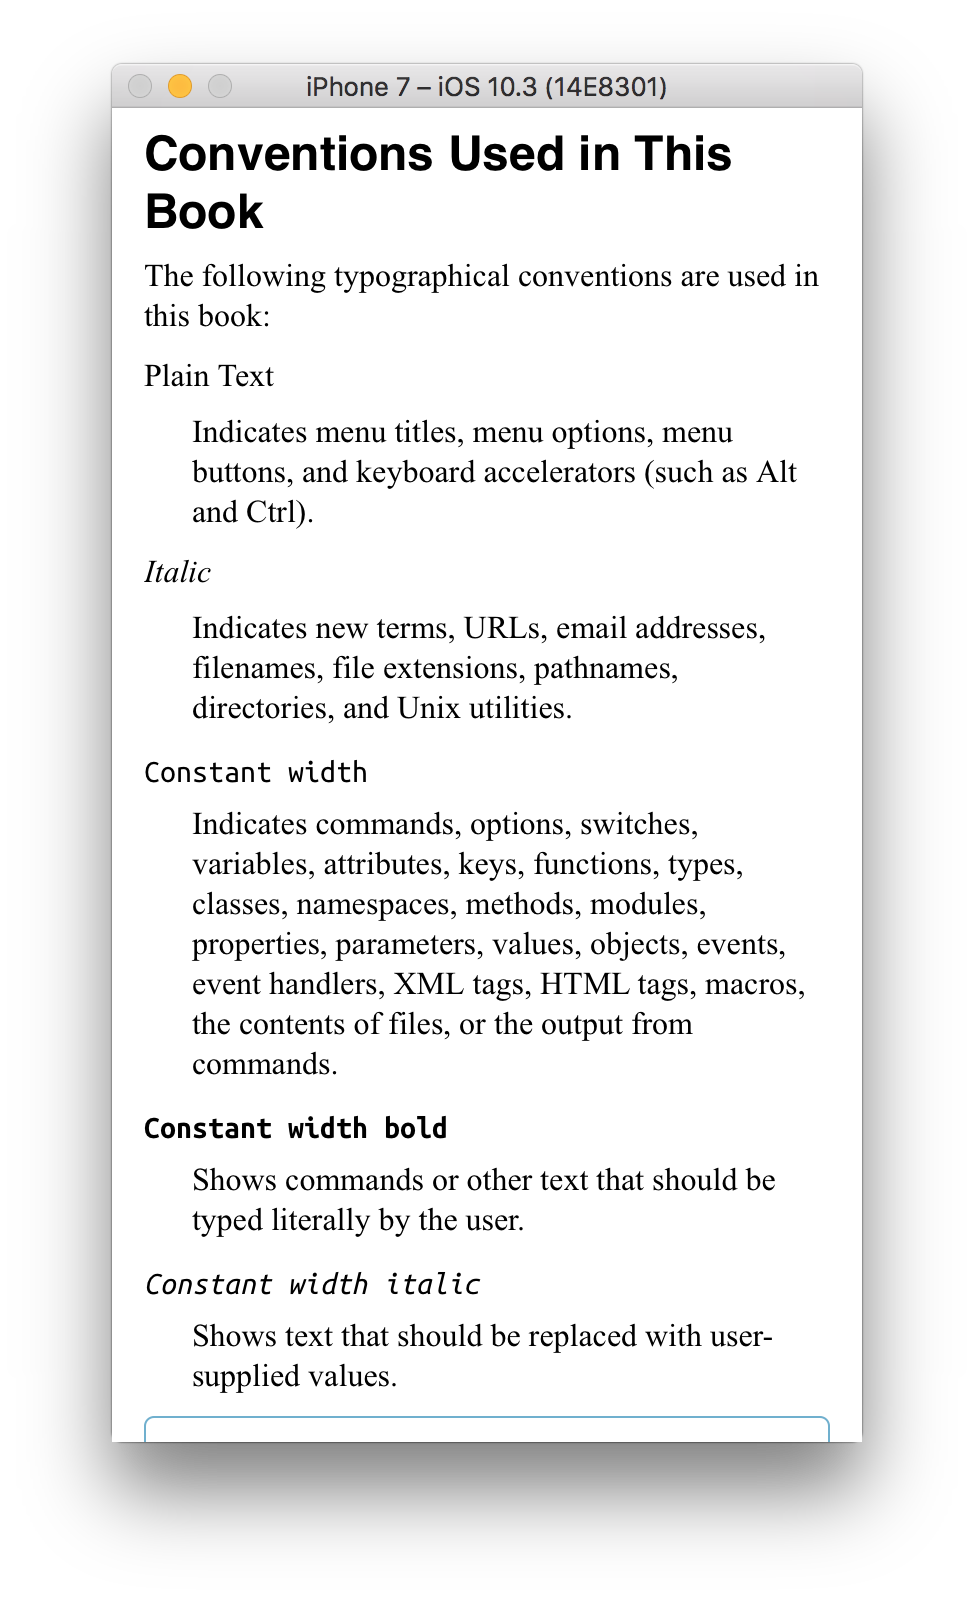
\includegraphics[width=.4\linewidth]{images/chapter-4-image-4-epubkit-view-scroll.png}
  \caption{Widok \texttt{EKViewController}}
  \label{chapter-4-image-4-epubkit-view-scroll}
\end{subfigure}%
\begin{subfigure}{.5\textwidth}
  \centering
  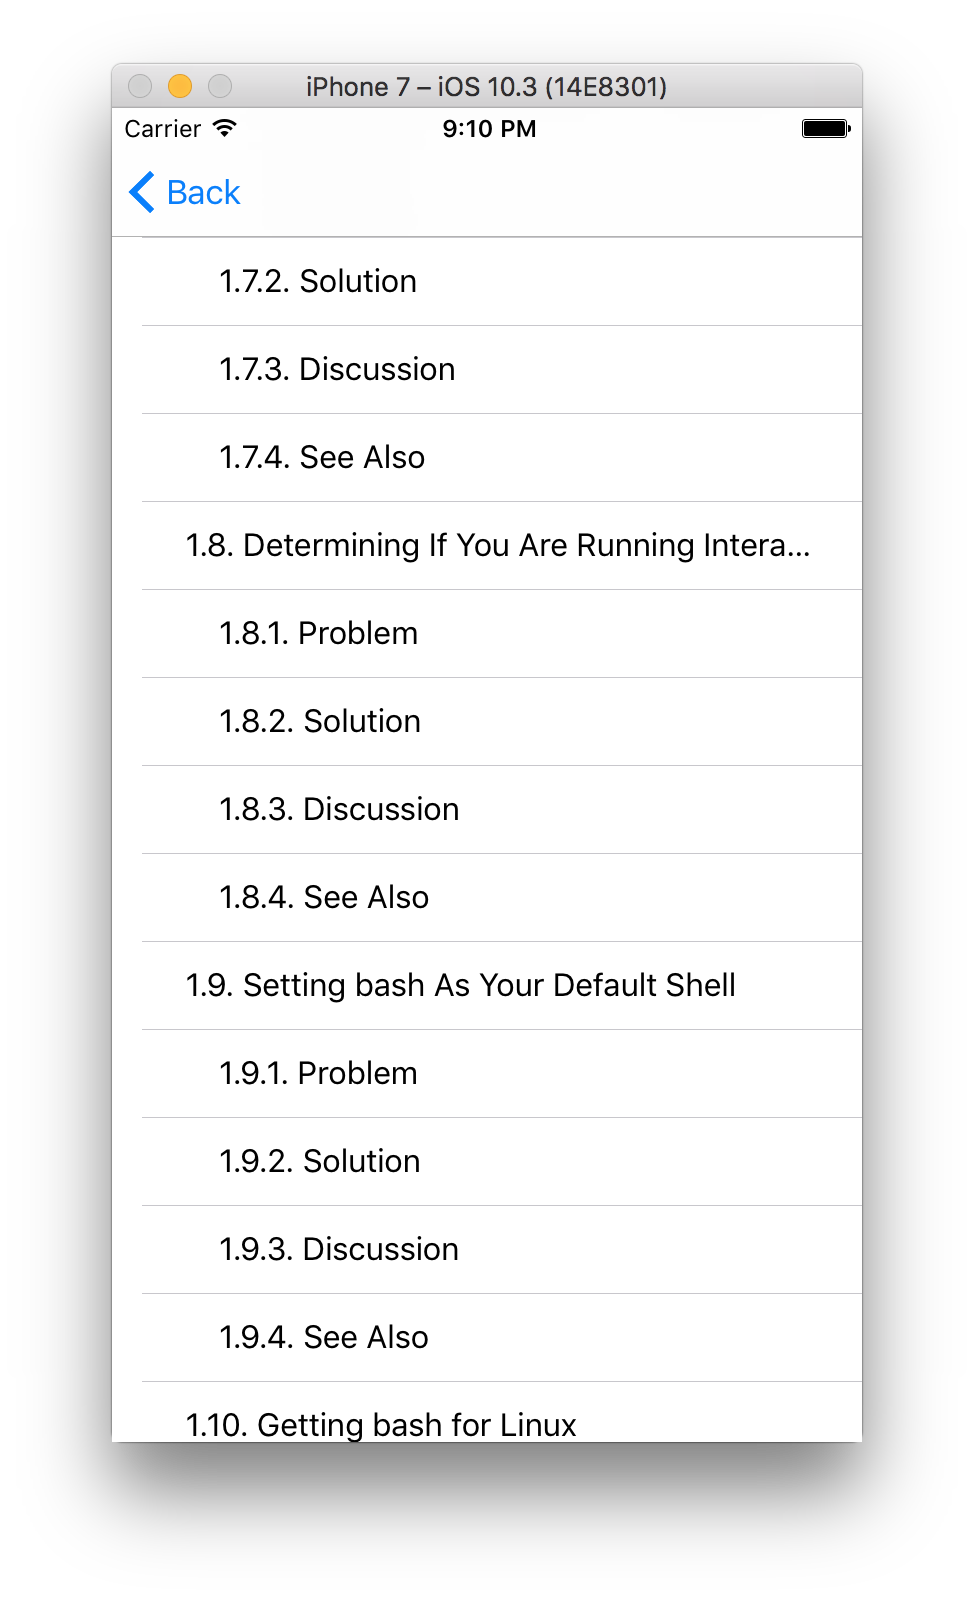
\includegraphics[width=.4\linewidth]{images/chapter-4-image-5-epubkit-view-toc.png}
  \caption{Widok \texttt{EKTableOfContentsViewController}}
  \label{chapter-4-image-5-epubkit-view-toc}
\end{subfigure}
\caption{Widoki dostępne w \textbf{EPUBKit}}
\label{chapter-4-image-4-5}
\end{figure}

Ostatnim elementem biblioteki \textbf{EPUBKit} jest jej widok. Jak wspomniano we wstępie do pracy, aby stworzyć widok znany z takich aplikacji jak \textit{iBooks} potrzeba wielu tygodni oraz ogromnego nakładu pracy wielu programistów. Jednak zdecydowałem się w obecnej wersji dostarczyć bardzo elementarny widok w celu zaprezentowania możliwości parsera oraz jak zręcznie można korzystać z klasy \texttt{EPUBDocument}. Widok ten będzie wyświetlał stronę w stylu \textit{Scrolling View} często spotykanym w systemach czytających, co oznacza, że zawartość całej książki zostanie wyświetlona w jednej kolumnie, a więc nie będzie podzielona na strony. Aby stworzyć widok, który dzielił by tekst na strony należało by dość mocno nadpisywać style dokumentu aby zapewnić \textit{paginację}, a następnie dostosować wyświetloną zawartość w formie widoku przypominającego książkę, czyli symulującego przerzucanie stron. Stworzenie tak zaawansowanego widoku pozostawiam na zaimplementowanie w którejś z przyszłych wersji biblioteki.

\begin{figure}[ht!]
  \centering
  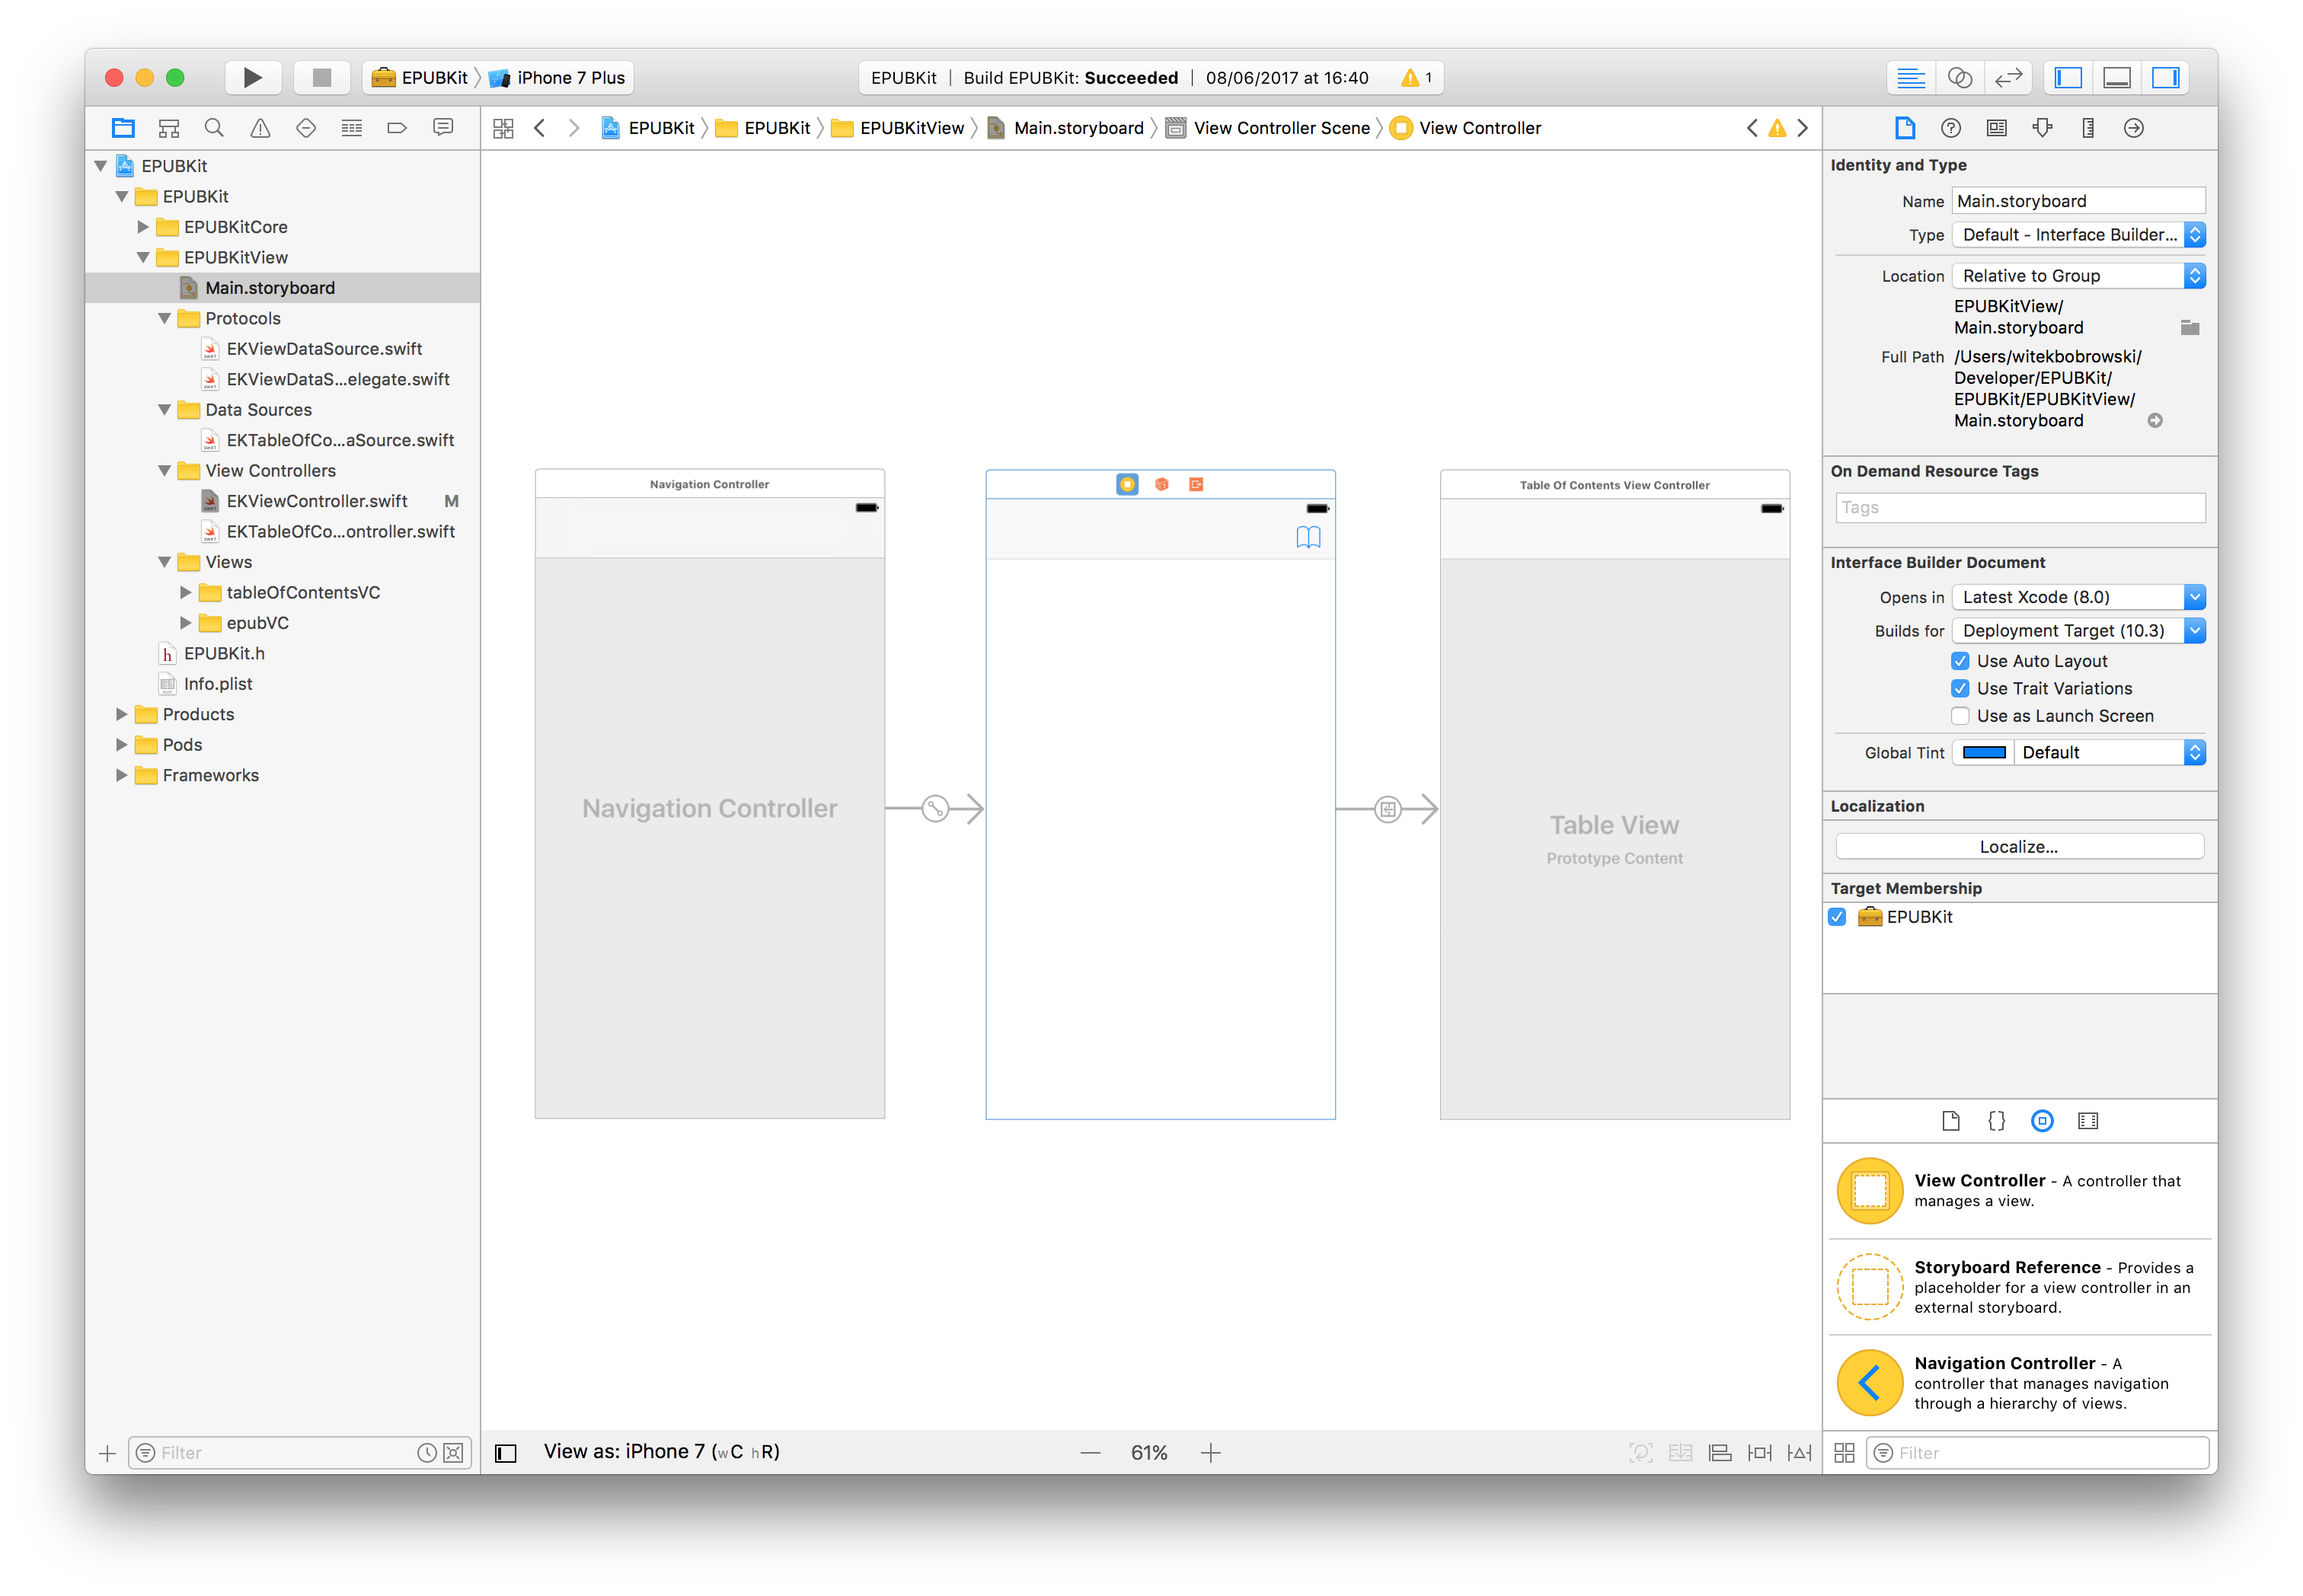
\includegraphics[width=120mm]{images/chapter-4-image-3-epubkit-storyboard.png}
  \caption{Plik \textit{Main.storyboard} biblioteki \textbf{EPUBKit} wyświetlony w Xcode}
  \label{chapter-4-image-3-epubkit-storyboard}
\end{figure}

Widok biblioteki \textbf{EPUBKit} w obecnej wersji ogranicza się do dwóch \textit{View Controller’ów} (czym są \textit{View Controllery} zostało objaśnione w rozdziale piątym przy okazji omawiania widoku aplikacji demonstracyjnej). Pierwszy z nich jest głównym widokiem w którym zostaje wyświetlony dokument, a drugi przedstawia spis treści, w którym po wybraniu pozycji jesteśmy przekierowani do odpowiedniego punktu w tekście. Na to wszystko składają się własne protokoły, klasy dostarczające dane (\textit{DataSource'y}), klasy i pliki \textit{Xib} widoków, dwie klasy dziedziczące po \texttt{UIViewController} oraz plik \textit{storyboard} w którym skomponowane są \textit{View Controller’y}.

\subsection{EKViewController}

Klasa reprezentuje główny \textit{View Controller} biblioteki, w którym zosatnie umieszczony widok dokumentu oraz, z którego będzie można przenieść się do spisu treści. Na wykazie \ref{EKViewController-declaration} przedstawiono deklarację klasy w której znaduje się referencja do elementu widoku typu \textit{UIView}, który został użyty w \textit{storyboardach} widocznych na rysunku \ref{chapter-4-image-3-epubkit-storyboard}.

\begin{lstlisting}[language=swift,caption={Deklaracja klasy texttt{EKViewController}},label=EKViewController-declaration]
public class EKViewController: UIViewController {
    @IBOutlet fileprivate weak var documentView: UIView!
    public var epubDocument: EPUBDocument?
    public override var prefersStatusBarHidden: Bool {
        return navigationController?.isNavigationBarHidden == true
    }
    public override var preferredStatusBarUpdateAnimation: UIStatusBarAnimation {
        return UIStatusBarAnimation.slide
    }

    public override func viewDidLoad() {
        super.viewDidLoad()
        configure()
    }
    public override func prepare(for segue: UIStoryboardSegue, sender: Any?) {
        if let tableOfContentsVC = segue.destination as? EKTableOfContentsViewController {
            tableOfContentsVC.delegate = self
            tableOfContentsVC.epubDocument = epubDocument
        }
    }
}
\end{lstlisting}

\texttt{EKViewController} deklaruje zmienną publiczną \texttt{epubDocument}, która posiada typ \texttt{EPUBDocument}. Przetrzymuje ona dokument który będzie wyświetlony, i należy go ustawić przed pojawieniem się widoku. Oznacza to, że programista musi samemu inicjalizować \texttt{EPUBDocument}, a następnie przekazać kontrolerowi \texttt{EKViewController} przed jego załadowaniem. Następnie zostają napisane dwie zmienne klasy nadrzędnej aby umożliwić chowania się paska nawigacji przy dotknięciu widoku. Ponieważ ten \textit{View Controller} jest osadzony w kontrolerze nawigacji \texttt{UINavigationController}, domyślnie wyświetlał on będzie pasek u góry ekranu służący do nawigacji. Będzie się na nim znajdować przycisk służący do powrotu do poprzedniego widoku, oraz dołączony został przycisk umożliwiający wyświetlenie spisu treści.

Aby przeprowadzić konfigurację \textit{View Controller’a}, nadpisuję metodę \texttt{viewDidLoad()} klasy nadrzędnej w celu wywołania własnej metody \texttt{configure()}, która jest zadeklarowana na rozszerzeniu widocznym na wykazie \ref{EKViewController-extension-1}. Ostatnią nadpisaną metodą jest \texttt{prepare(for:sender:)}, która zostaje wywołana w przypadku gdy jeden \textit{View Controller} będzie próbował przejść do kolejnego, w tym wypadku będzie to sytuacja gdy użytkownik naciśnie przycisk wyświetlający spis treści.

\begin{lstlisting}[language=swift,caption={Rozszerzenie klasy texttt{EKViewController} o metody konfiguracji},label=EKViewController-extension-1]
//MARK: - Configuration
extension EKViewController {
    fileprivate func configure() {
        let nibName = String(describing: EKInfiniteScrollView.self)
        let nib = UINib(nibName: nibName, bundle: Bundle(for: EKInfiniteScrollView.classForCoder()))
        let infiniteScrollView = nib.instantiate(withOwner: EKInfiniteScrollView.self, options: nil).first as! EKInfiniteScrollView
        view.addSubview(infiniteScrollView)
        documentView = infiniteScrollView
        infiniteScrollView.epubDocument = epubDocument
        navigationController?.navigationBar.barTintColor = .white
        navigationController?.navigationBar.shadowImage = UIImage()
        let tapGestureRecogniser = UITapGestureRecognizer(target: self, action: #selector(hideNavigationBar(_:)))
        view.addGestureRecognizer(tapGestureRecogniser)
    }
    @objc private func hideNavigationBar(_ sender: UITapGestureRecognizer){
         navigationController?.setNavigationBarHidden(navigationController?.isNavigationBarHidden == false, animated: true)
    }
}
\end{lstlisting}

W pierwszym rozszerzeniu klasy, definiuję metodę \texttt{configure()}, w której przeprowadzam konfigurację jej widoków. Inicjalizuję z pliku \textit{Xib} widok w którym zostanie wyświetlony dokument, a następnie przypisuje do zmiennej \texttt{documentView} oraz dodaję jako pod-widok głównego widoku i przekazuję dokument EPUB w postaci zmiennej \texttt{epubDocument}. Pod koniec dodaję do głównego widoku \texttt{tapGestureRecogniser}, który jest instancją klasy odpowiedzialnej za rozpoznawanie wykonanego przez użytkownika gestu dotknięcia na ekran. Podczas inicalizacji \texttt{UITapGestureRecognizer} przekazuje mu niżej zadeklarowaną metodę \texttt{hideNavigationBar(\_:)}, która zostanie przez niego wywołana w momencie rozpoznania gestu. Metoda ta chowa lub pokazuje pasek nawigacji tak jak jest to widoczne na rysunku \ref{chapter-4-image-4-epubkit-view-scroll}.

\begin{lstlisting}[language=swift,caption={Rozszerzenie klasy texttt{EKViewController} o protokół texttt{EKTableOfContentsViewControllerDelegate}},label=EKViewController-extension-2]
//MARK: - EKTableOfContentsViewControllerDelegate
extension EKViewController: EKTableOfContentsViewControllerDelegate {
    func tableOfContentsView(_ tableOfContentsView: EKTableOfContentsViewController, didSelectRowAt indexPath: IndexPath) {
        if let infiniteScrollView = documentView as? EKInfiniteScrollView {
            infiniteScrollView.idOfElementToDisplay = (tableOfContentsView.dataSource.item(at: indexPath) as? EKTableOfContentsDataSource.Item)?.item
        }
    }
}
\end{lstlisting}

Drugim i ostatnim rozszerzeniem widocznym na wykazie \ref{EKViewController-extension-2}, stosuję na klasie protokół \texttt{EKTableOfContentsViewControllerDelegate}, który jest własnym protokołem stworzonym w celu zdefiniowania delegata dla \texttt{EKTableOfContentsViewController}. Protokół ten wymaga implementacji metody \texttt{tableOfContentsView(\_:didSelectRowAt:)}. Wzorzec projektowy \textbf{Delegat} jest wyjątkowo często stosowanym wzorcem przy programowaniu na iOS. Większość klas należących \textit{iOS SDK} deklaruje swoich delegatów (w formie protokołu), a każdy z nich posiada szereg metod, które musi lub może zaimplementować przy stosowaniu protokołu.

\subsection{EKTableOfContentsViewController}

Widok wiczony na rysunku \ref{chapter-4-image-5-epubkit-view-toc} wyświetla spis treści dokumentu \texttt{EPUBDocument} i jest reprezentowany przez klasę \texttt{EKTableOfContentsViewController}.

\begin{lstlisting}[language=swift,caption={Deklaracja klasy \texttt{EKTableOfContentsViewController}},label=EKTableOfContentsViewController-declaration]
class EKTableOfContentsViewController: UIViewController {
    @IBOutlet fileprivate weak var tableView: UITableView!
    public weak var delegate: EKTableOfContentsViewControllerDelegate?
    public var dataSource = EKTableOfContentsDataSource()
    public var epubDocument: EPUBDocument? {
        didSet {
            dataSource.epubDocument = epubDocument
        }
    }
    override func viewDidLoad() {
        super.viewDidLoad()
        configure()
    }
}
\end{lstlisting}

\texttt{EKTableOfContentsViewController} deklaruje referencję do elementu w \textit{storyboardach} własnego delegata, oraz dotąd niespotkany w pracy \textit{dataSource}. Kod źródłowy oraz jego rola zostaną omówione w podrozdziale 4.3.4, który będzie własnie tej klasie zadedykowany. Po raz kolejny do widoku przypisana jest instancja \texttt{EPUBDocument}, z której widok ten czerpie dane, a zmienna do której jest przypisana, posiada tak zwany \textit{Obserwator własności} (z ang. Property Observer), czyli blok \textit{didSet\{ \ldots \}}, który zostanie wywołany w przypadku gdy wartość własności się zmieni. Istnieje drugi obserwator, jakim jest \textit{willSet\{ \ldots \}}, ten natomiast wywoływany tuż przed zmianą wartości przez własność. W blokach tych istnieje możliwość wykorzystania specjalnej stałej \texttt{newValue} lub \texttt{oldValue} w zależności od rodzaju obserwatora, co daje możliwość dostępu do wartości, która zostanie zmieniona, lub zostanie przypisana. w Tym wypadku, gdy wartość do zmiennej \texttt{epubDocument} zostanie przypisana, zostanie wykonana instrukcja \texttt{dataSource.epubDocument = epubDocument}, czyli przypisanie samej siebie do własności zmiennej \textit{dataSource} o tej samej nazwie.

\begin{lstlisting}[language=swift,caption={Rozszerzenie klasy \texttt{EKTableOfContentsViewController} o metodę konfiguracji},label=EKTableOfContentsViewController-exension-1]
//MARK: - Configuration
extension EKTableOfContentsViewController {
    fileprivate func configure() {
        navigationController?.navigationBar.barTintColor = .white
        navigationController?.navigationBar.shadowImage = UIImage()
        navigationController?.navigationBar.backItem?.title = ""
        dataSource.delegate = self
        tableView.dataSource = dataSource
        tableView.delegate = self
        tableView.register(UINib(nibName: "EKTableOfContentsViewCell", bundle: Bundle(for: classForCoder)), forCellReuseIdentifier: "EKTableOfContentsViewCell")
    }
}
\end{lstlisting}

Konfiguracja klasy jest przeprowadzona w podobnym stylu co w poprzednim przypadku, i tak też będzie w kolejnych. Rozdzielenie kodu klasy jest praktyką mającą na celu pilnowanie porządku oraz rozczłonowanie deklaracji na fragmenty odpowiedzialne za konkretne czynności. Wykaz \ref{EKTableOfContentsViewController-exension-1} deklaruje metodę konfiguracji, która zostaje wywołana w momencie załadowania widoku. Konfiguruje ona widok paska nawigacji, oraz ustawie siebie (\texttt{self}) jako delegata tabeli oraz źródła danych. Na końcu tabela rejestruje widoki, które będzie mogła wykorzystać jako komórki. Klasa widoku komórki \texttt{EKTableOfContentsViewCell} jest bardzo prosta, ponieważ jedyne co zawiera to referencję etykiety, na której zostanie wyświetlona nazwa podrozdziału oraz rozszerzenie o trywialną metodę konfigurującą.

\begin{lstlisting}[language=swift,caption={Rozszerzenie klasy \texttt{EKTableOfContentsViewController} o protokoły \texttt{UITableViewDelegate} oraz \texttt{EKViewDataSourceDelegate}},label=EKTableOfContentsViewController-exension-2]
//MARK: - UITableViewDelegate
extension EKTableOfContentsViewController: UITableViewDelegate {
    func tableView(_ tableView: UITableView, didSelectRowAt indexPath: IndexPath) {
        delegate?.tableOfContentsView(self, didSelectRowAt: indexPath)
        navigationController?.popViewController(animated: true)
    }
}
//MARK: - EKViewDataSourceDelegate
extension EKTableOfContentsViewController: EKViewDataSourceDelegate {
    func dataSourceDidFinishBuilding(_ dataSource: EKViewDataSource) {
        tableView.reloadData()
    }
}
\end{lstlisting}

Jeżeli skonfigurowano kontroler \texttt{EKTableOfContentsViewController} jako delegata, musi on więc stosować jego protokół. Jak zademonstrowano na wykazie \ref{EKTableOfContentsViewController-exension-2} zastosowano protokoły \texttt{UITableViewDelegate} oraz \texttt{EKViewDataSourceDelegate} w celu zaimplementowania ich metod. Pierwsza z nich, metoda \texttt{tableView(\_:didSelectRowAt:)} zostaje wywołana w momencie naciśnięcia na dany rząd w tabeli, którą podaje jako parametr, przez użytkownika. Jako parametr podaje również indeks rzędu, który reprezentowany jest strukturą \texttt{IndexPath}, którego następnie użyjemy przy okazji wywołania metody na delegacie, aby jej przekazać index. Delegat, którym w tym przypadku jest \texttt{EKViewController}, otrzyma indeks i z jego pomocą wyciągnie z \texttt{dataSource} odpowiednią informację w celu wyświetlenia pożądanego przez użytkownika fragmentu w tekście.

Drugą metodą jest \texttt{dataSourceDidFinishBuilding(\_:)}, która powiadamia delegata (czyli w tym przypadku \texttt{EKTableOfContentsViewController}) o tym aby wymusił przeładowanie danych na tabeli, ponieważ źródło danych zostało zbudowane, i jest gotowe dostarczać je widokowi.

\subsection{EKInfiniteScrollView}

\texttt{EKInfiniteScrollView} (wykaz ref{EKInfiniteScrollView-declaration}) jest jedynym prototypowym widokiem dostarczonym w tej wersji EPUBKit, który potrafi wyświetlić dokument EPUB. Widok w tym stylu jest często spotykany w czytnikach, więc to jego zdecydowałem się zaimplementować w pierwszej kolejności.

\begin{lstlisting}[language=swift,caption={Deklaracja klasy \texttt{EKInfiniteScrollView}}, label=EKInfiniteScrollView-declaration]
class EKInfiniteScrollView: UIView {
    @IBOutlet fileprivate weak var contentView: UIView!
    fileprivate var webView: WKWebView!
    public var epubDocument: EPUBDocument? {
        didSet {
            if let epubDocument = epubDocument {
                configure(with: epubDocument)
            }
        }
    }
    public var idOfElementToDisplay: String? {
        didSet {
            guard let id = idOfElementToDisplay else { return }
            if id.contains("#") {
                let idSubstring = id.substring(from: id.characters.index(of: "#")!)
                webView.evaluateJavaScript("location.href = \"\(idSubstring)\";")
            } else {
                webView.evaluateJavaScript("location.href = \"#\(id)\";")
            }
        }
    }
    override func awakeFromNib() {
        super.awakeFromNib()
        configure()
    }
}
\end{lstlisting}

Klasa ta dziedziczy po \texttt{UIView}, czyli najbardziej podstawowej klasie reprezentującej widok. \texttt{EKInfiniteScrollView} deklaruje pod-widok, który jest kontenerem dla drugiego pod-widoku, którego typem jest \texttt{WKWebView}. Typ ten reprezentuje widok, który pozwala na wyświetlanie treści w technologiach internetowych, takich jak pliki \textit{HTML} stylizowane plikami \textit{CSS}. Ze względu na to, iż dokument EPUB między innymi zbudowany jest w oparciu o te technologie można przy pomocy \texttt{WKWebView} wyświetlić jego zawartość. Należy jednak zmodyfikować nieco zawartość dokumentu w celu otrzymania pożądanego widoku. \texttt{EKInfiniteScrollView} posiada również zmienną, do której może zostać przypisana referencja do instancji \texttt{EPUBDocument} (typ opcjonalny), a w momencie jej przypisania zostanie sprawdzona wartość i w przypadku gdy jest ona niepusta, zostaje wywołana metoda konfigurująca widok. Kolejną zmienna jest \texttt{idOfElementToDisplay}, własność służąca do wywoływania nawigacji w przypadku jej nadpisania do określonego elementu w wyświetlanym dokumencie. Ze względu na to, że widok jest stwrzony w pliku \textit{Xib}, ogólną metodę konfiguracyjną wywołuję w napisanej metodzie \texttt{awakeFromNib()}. Metoda ta jest wywołana w momencie zainicjalizowania widoku oraz wszystkich elementów z pliku \textit{Xib}, dzięki czemu mamy gwarancję, że elementy konfigurowane są już w pełni zainicjalizowane.


\begin{lstlisting}[language=swift,caption={Rozszerzenie klasy \texttt{EKInfiniteScrollView} o metody konfiguracji}, label=EKInfiniteScrollView-extension-1]
//MARK: - Configuration
extension EKInfiniteScrollView {
    fileprivate func configure() {
        webView = WKWebView(frame: contentView.frame)
        constrainView(view: webView, toView: contentView)
        webView.allowsBackForwardNavigationGestures = false
        webView.scrollView.showsHorizontalScrollIndicator = false
        webView.scrollView.pinchGestureRecognizer?.isEnabled = false
        webView.navigationDelegate = self
        webView.scrollView.delegate = self
    }
    public func configure(with epubDocument: EPUBDocument){
        var htmlString = "<html><body>"
        for spineItem in epubDocument.spine.items {
            if let manifestItem = epubDocument.manifest.items[spineItem.idref] {
                htmlString.append("<div id=\"\(manifestItem.path)\"></div>")
                let itemURL = epubDocument.contentDirectory.appendingPathComponent(manifestItem.path)
                let spineHtmlString = (try? String(contentsOf: itemURL)) ?? ""
                htmlString.append(spineHtmlString)
            }
        }
        htmlString += "</html></body>"
        webView.loadHTMLString(htmlString, baseURL: epubDocument.contentDirectory)
    }
    fileprivate func constrainView(view:UIView, toView contentView: UIView) {
        contentView.addSubview(view)
        view.translatesAutoresizingMaskIntoConstraints = false
        view.leadingAnchor.constraint(equalTo: contentView.leadingAnchor).isActive = true
        view.topAnchor.constraint(equalTo: contentView.topAnchor).isActive = true
        view.trailingAnchor.constraint(equalTo: contentView.trailingAnchor).isActive = true
        view.bottomAnchor.constraint(equalTo: contentView.bottomAnchor).isActive = true
    }
}
\end{lstlisting}

Podstawowa metoda konfiguracji \texttt{configure()} stylizuje widoki w pliku \textit{Xib}, oraz przypisuje siebie jako delegata widokowi wyświetlającemu publikację oraz jego pod-widokowi o typie \texttt{UIScrollView}. Druga metoda konfiguruje widok na podstawie przekazanego dokumentu EPUB. Zgodnie z jego specyfikacją, zbierze wszystkie elementy manifestu wymienione w kolejności określone w \textit{kręgosłupie} czyli \textit{spine}. Aby wyświetlić dokument w całości trzeba scalić wszystkie elementy dokumentu razem, w formie \texttt{stringa}, aby następnie załadować je w \texttt{webView} przy użyciu metody \texttt{loadHTMLString(\_:baseURL:)}. Podczas konkatynacji każdego z elementów, dorzucam do wyniku element \texttt{div}, który zapewni prawidłową nawigację po dokumencie. Ostatnia metodą konfiguracyjna pozwala na \textit{przyczepienie} jednego widoku do drugiego przy pomocy \textit{constraints}, które służą do ustalania odległości elementów interfejsu między sobą.


\begin{lstlisting}[language=swift,caption={Rozszerzenie klasy \texttt{EKInfiniteScrollView} o protokoły \texttt{WKNavigationDelegate} oraz \texttt{UIScrollViewDelegate}}, label=EKInfiniteScrollView-extension-2]
//MARK: - WKNavigationDelegate
extension EKInfiniteScrollView: WKNavigationDelegate {
    func webView(_ webView: WKWebView, didCommit navigation: WKNavigation!) {
        webView.evaluateJavaScript("var meta = document.createElement('meta');meta.setAttribute('name', 'viewport');meta.setAttribute('content', 'width=device-width, initial-scale=1.0, minimum-scale=1.0, maximum-scale=1.0, user-scalable=no');document.getElementsByTagName('head')[0].appendChild(meta);")
    }
}
//MARK: - UIScrollViewDelegate
extension EKInfiniteScrollView: UIScrollViewDelegate {
    func scrollViewDidScroll(_ scrollView: UIScrollView) {
        if scrollView.contentOffset.x != 0 {
            scrollView.contentOffset.x = 0
        }
    }
}
\end{lstlisting}

\texttt{EKInfiniteScrollView} dzięki swojej delegacji w pod-widokach, deklaruje ważne dla niego czynności w metodach protokołów. Pierwsza z nich jest wywoływana gdy \texttt{webView} otrzyma polecenie nawigacji do strony, czyli rozpocznie proces jej ładowania. W tym czasie delegat załaduje \textit{javascript}, którym zmodyfikuje styl wyświetlanej strony. Ustawi jej odpowiednią szerokość oraz zabroni przybliżania lub oddalania, aby widok był statyczny. Druga metoda również zablokuje możliwość przesuwania w wypadku gdyby rozmiar zawartości strony przekraczaj z jakiegoś względu oczekiwane wymiary. W ten sposób otrzymujemy efekt widoczny na rysunku \ref{chapter-4-image-4-epubkit-view-scroll}. Nie jest to rozwiązanie idealne, i zapewne brakuje mu kilku funkcjonalności znanych z takich czytników jak \textit{iBooks}, lecz jak na wersje pierwszą biblioteki, jest zdecydowanie wystarczający. Przewiduję ulepszenie widoku w kolejnych wersjach biblioteki.

\subsection{EKTableOfContentsDataSource}

\textit{Data source} jest stosowany w wielu klasach widoku znajdujących się w \textit{iOS SDK}. Ich celem jest dostarczenie modelu dla widoku, którego struktura będzie do niego dopasowana. Zadaniem jego jest zebranie danych, organizacja ich w określony sposób i zbudowanie na ich podstawie modelu.

\begin{lstlisting}[language=swift,caption={Deklaracja klasy \texttt{EKTableOfContentsDataSource}}, label=EKTableOfContentsDataSource-declaration]
class EKTableOfContentsDataSource: NSObject {
    public weak var delegate: EKViewDataSourceDelegate?
    public var epubDocument: EPUBDocument? {
        didSet {
            if epubDocument != nil {
                build(from: epubDocument!)
            }
        }
    }
    fileprivate var model: [[Item]] = []
    struct Item {
        let item: String
        let title: String
    }
}
\end{lstlisting}

Takim źródłem danych (\textit{z ang. data source}) jest klasa \texttt{EKTableOfContentsDataSource}, dostarczająca model danych widokowi odpowiedzialnemu za spis treści. Klasa ta (wykaz \ref{EKTableOfContentsDataSource-declaration}) deklaruje swojego delegata, własne źródło danych jakim jest instancja \texttt{EPUBDocument} oraz własność \textit{model}, której struktura jest skomponowana w sposób taki aby pasowała do tabeli, którą bedzie zasiedlała. Ponieważ tabela w postaci klasy \texttt{UITableView}, składa się z sekcji, które posiadają swoje rzędy, typem modelu jest tablica tablic typu własnego \texttt{Item}. Typ ten reprezentuje pojedyńczy rząd, a tablica w której się znajduje reprezentuje jedną sekcje. Ze względu na to iż sekcji może w tabeli być wiele, umieszczamy sekcję w tablicy i w ten sposób typem modelu źródła danych jest \texttt{[[Item]]}.

\begin{lstlisting}[language=swift,caption={Rozszerzenie klasy \texttt{EKTableOfContentsDataSource} o protokół \texttt{EKViewDataSource}}, label=EKTableOfContentsViewController-extension-1]
//MARK: - EKViewDataSource
extension EKTableOfContentsDataSource: EKViewDataSource {
    func build(from epubDocument: EPUBDocument) {
        var section: [Item] = []
        func evaluate(tableOfContents: [EPUBTableOfContents], space: String) {
            for item in tableOfContents {
                section.append(Item(item: item.item ?? "" , title: space + item.label))
                if let children = item.subTable {
                    evaluate(tableOfContents: children, space: space + "    ")
                }
            }
        }
        if let children = epubDocument.tableOfContents.subTable {
            evaluate(tableOfContents: children, space: "")
        }
        self.model = [section]
    }
    public func item(at indexPath: IndexPath) -> Any {
        return model[indexPath.section][indexPath.row]
    }
}
\end{lstlisting}

Podążając ustalonymi konwencjami (mowa o własnych protokołach, szczegółowo omówionych w kolejnym podrozdziale) rozszerzam klasę \texttt{EKTableOfContentsDataSource} o protokół \texttt{EKViewDataSource} co wymusza implementację jego metod. Metoda budująca model będzie analizowała każdą pozycję we własnośći \texttt{tableOfContents} instancji \texttt{EPUBDocument}, aby otrzymać jej tytuł oraz referencję do pliku w strukturze dokumentu. Aby przeszukać spis treści w głąb, zaimplementowałem dodatkową metodę, która dzięki rekurencji dotrze do każdego elementu w strukturze. Aby ta głębokość została odwzorowana w widoku, przekazuję funkcji pusty \texttt{string}, który następnie z każdym poziomem zostaje powiększony o kilka znaków spacji aby tytuł był odpowiednio odsunięty, co pozwoli na lepszą orientację użytkownika w strukturze dokumentu. Druga metoda tego protokołu będzie natomiast zwracać element w określonych sekcji i rzędzie modelu.

\begin{lstlisting}[language=swift,caption={Rozszerzenie klasy \texttt{EKTableOfContentsDataSource} o protokół \texttt{UITableViewDataSource}}, label=EKTableOfContentsViewController-extension-2]
//MARK: - UITableViewDataSource
extension EKTableOfContentsDataSource: UITableViewDataSource {
    func numberOfSections(in tableView: UITableView) -> Int {
        return model.count
    }
    func tableView(_ tableView: UITableView, numberOfRowsInSection section: Int) -> Int {
        return model[section].count
    }
    func tableView(_ tableView: UITableView, cellForRowAt indexPath: IndexPath) -> UITableViewCell {
        let chapter = item(at: indexPath) as! Item
        let cell = tableView.dequeueReusableCell(withIdentifier: "EKTableOfContentsViewCell" ,
                                                 for: indexPath) as! EKTableOfContentsViewCell
        cell.configure(with: chapter.title)
        return cell
    }
}
\end{lstlisting}

Ostatnim protokołem stosowanym przez to źródło danych jest \texttt{UITableViewDataSource}, który wymaga zaimplementowania metod, dzięki którym tabela dowiaduje się, jakie dane modelu będą znajdowały się w danym miejscu. Pierwszą rzeczą o którą pyta \texttt{UITableView} swojego delegata, to ile w modelu znajduje się sekcji. Delegat, czyli klasa \texttt{EKTableOfContentsDataSource} zwróci tabeli \texttt{model.count}, czyli ilość elementów w najwyższej tablicy. Gdy tabela dowię się ile będzie musiała wyświetlić sekcji, zapyta metodą \texttt{tableView(\_:numberOfRowsInSection:)} o ilość rzędów w sekcji, którą podaje jako parametr, a delegat odpowie: \texttt{model[section].count}, a więc zwróci ilość elementów w podrzędnej tablicy. Ostatnią wymaganą metodą przez protokół jest zapytanie o komórkę którą ma wyświetlić w danym rzędzie. Zanim zwrócimy komórkę o odpowiednim typie tabeli, należy przy pomocy parametru indeksu wyciągnąć z modelu metodą \texttt{item(at:)} odpowiedni element i skonfigurować nim komórkę. Ze względów wydajnościowych, tabela posiada funkcję kolejkowania komórek, które nie znajdują się na ekranie w celu ich ponownego użycia. W ten sposób nawet w przypadku ogromnej ilośc danych tabela może operować zaledwie kilkoma komórkami, które wciąż uzupełnia nowymi danymi. Więc metoda \texttt{dequeueReusableCell(withIdentifier:for:)} pozwoli nam uzyskać taką komórkę ze wspólnej puli, i w końcu skonfigurować ją odpowiednim elementem i finalnie ją zwrócić.

Systemowe klasy takie jak \texttt{UITableView} czy \texttt{UICollectionView}, to potężne elementy widoku wykorzystywane w praktycznie każdej aplikacji, a prawidłowe ich wykorzystanie jest kluczem do stworzenia szybkiej i wydajnej aplikacji. Na przykładzie klasy \texttt{UITableViewDataSource} widać jak dobrze zorganizowany i zaprojektowany kod jest kluczowy w prawidłowym działaniu aplikacji. Podążając wytycznymi, trzymamy się ścieżki wyznaczonej w celu utrzymania stabilności oraz uzyskania jak największej wydajności i niezawodności kodu.

\subsection{Protokoły}

Widok \textbf{EPUBKit} deklaruje własne protokoły pomocnicze, aby przyjąć pewne normy, które będą musiały zostać uszanowane przez nowo powstające klasy. Podejście te zapewnia spójność kodu pośród określonego rodzaju klas, lecz co najważniejsze, pozwala to na przyjęcie pewnych konwencji obowiązujących w projekcie. Każdy z poniższych protokołów oznaczony jest słowem kluczowym \textit{class}, więc stosować je będą mogły wyłącznie klasy.

\begin{lstlisting}[language=swift,caption={Deklaracja protokołu \texttt{EKViewDataSource}}, label=EKViewDataSource-declaration]
protocol EKViewDataSource: class {
    func build(from epubDocument: EPUBDocument)
    func item(at indexPath: IndexPath) -> Any
}
\end{lstlisting}

Wykaz \ref{EKViewDataSource-declaration} przedstawia deklarację protokołu \texttt{EKViewDataSource}, który powinien być stosowany przez każdą klasę która pełni rolę źródła danych w bibliotece \textbf{EPUBKit}. Na ten moment definiuje on dwie metody, pierwsza z nich jest metodą w której z założenia ma się odbywać budowanie z instancji \texttt{EPUBDocument}. Druga powinna zwracać obiekt znajdujący się na pozycji określonej przez indeks w formie instancji \texttt{IndexPath}.

\begin{lstlisting}[language=swift,caption={Deklaracja protokołu \texttt{EKViewDataSourceDelegate}}, label=EKViewDataSourceDelegate-declaration]
protocol EKViewDataSourceDelegate: class {
    func dataSourceDidFinishBuilding(_ dataSource: EKViewDataSource)
}
\end{lstlisting}

Kolejnym protokołem jest delegatem klasy stosującej protokół \texttt{EKViewDataSource}. Protokół \texttt{EKViewDataSourceDelegate} którego implementacja przedstawiona na wykazie \ref{EKViewDataSourceDelegate-declaration} definiuję metodę wywoływaną przez źródło danych na delegacie w momencie ukończenia budowy modelu. To pozwala na reakcję ze strony delegata, tak jak miało to miejsce w klasie \texttt{EKTableOfContentsViewController}, która wymuszała przeładowanie danych w tabeli.

\begin{lstlisting}[language=swift,caption={Deklaracja protokołu \texttt{EKTableOfContentsViewControllerDelegate}}, label=EKTableOfContentsViewControllerDelegate-declaration]
protocol EKTableOfContentsViewControllerDelegate: class {
    func tableOfContentsView(_ tableOfContentsView: EKTableOfContentsViewController, didSelectRowAt indexPath: IndexPath)
}
\end{lstlisting}

\section{Dystrybucja}

Ta część będzie opisywała najpopularniejsze metody dystrybucji biblioteki na iOS. Najczęściej dystrybucja odbywa się poprzez menadżery paczek (and. \textit{Package Manager}), ponieważ traktowanie dodatkowych bibliotek czy narzędzi jako paczki czy moduły jest bardzo wygodną konwencją. Systemy takie jak \texttt{CocoaPods} czy \texttt{Carthage} wykorzystują jeden plik w którym programista może deklarować wykorzystywane moduły, a po wykonaniu odpowiedniej komendy moduły te zostaną pobrane z bazy menadżera paczek dołączone do przestrzeni roboczej dzięki czemu będą dostępne do użycia w plikach źródłowych projektu poprzez zaimportowanie ich tak jak zademonstrowano to na wykazie \ref{import}.

\begin{lstlisting}[language=swift-reference,caption={Sposób importowania dodatkowego modułu},label=import]
import (module)
\end{lstlisting}

Bardzo często zdarza się, że biblioteki w celach zyskania popularności zostają udostępnione bezpośrednio na portalu GitHub, w którym prezentowane są sposoby instalacji, oraz demonstracja API. Udostępnianie w tym miejscu swojej biblioteki jest dobrym pomysłem ze względu na to, że programiści zainteresowani jej wykorzystaniem mają wgląd w jej kod źródłowy jeszcze zanim dołączą ją do swojego projektu przy pomocy menadżerów. GitHub pozwala na tak zwane \textit{forkowanie} repozytorium, co oznacza przypisanie go do swojego profilu wraz z całą historią systemu kontroli wersji. W ten sposób każdy może zaimplementować własne funkcjonalności a następnie poprosić właściciela repozytorium o dołączenie ich do głównej gałęzi repozytorim za pomocą \textit{pull-request}. Społeczność open-source na GitHub'ie jest obecna, i w momencie podchwycenia popularności przez repozytorium, niezależni programiści często dostosowują je pod swoje potrzeby a potem często prezentują zmiany, które mogą zostać zatwierdzone przez właściciela. System kontroli wersji pozwala na używanie modułów więc istnieje możliwość wykorzystania publicznie dostępnych bibliotek z GitHub'a bez integracji projektu z którymś z menadżerów paczek.

Aby udostępnić projekt na GitHubie jedyne co potrzebujemy to własny profil oraz repozytorium lokalne w którym znajduje się projekt. Jest to oczywiście najprostsze rozwiązanie, chociaż w innych przypadkach wcale nie jest to skomplikowane. Sprowadza się to zazwyczaj do wykonania pewnych poleceń z lini komend oraz wykonania innych równie trywialnych czynności. Dobrą praktyką jest udostępnianie biblioteki na GitHubie oraz na wszyskich możliwych menadżerach paczek, zapewni to instalację w każdym projekcie niezależnie z jakim menadżerem jest zintegrowany. Niewątpliwie taki los czeka bibliotekę EPUBKit, która została stworzona z myślą o udostępnieniu jej publicznie.

Biblioteka \textbf{EPUBKit} została udostępniona na portalu GitHub pod adresem url: \url{https://github.com/witekbobrowski/EPUBKit}. Jest również dostępna do zainstalowania przy pomocy CocoaPods po dołączeniu jej w pliku \textit{Podfile}. Sczegóły instalacji i wykorzystania w kolejnym rozdziale.
